% Dokumentenklasse fuer Artikel waehlen
\documentclass[12pt,onecolumn,oneside,titlepage]{article}

% Deutsche Grundeinstellungen und DIN A4
\usepackage{a4}

% Zur Einbindung von Grafiken mit \includegraphics
\usepackage[pdftex]{graphicx,color}
\DeclareGraphicsExtensions{.pdf,.jpg,.png,.eps,.ps}
\usepackage{graphicx}
\graphicspath{ {images/} }

\usepackage{textcomp,upquote,lmodern,listings}
\usepackage{subcaption}
\usepackage{float}

% Bibliographie mit BibTeX
%\usepackage{natbib}

% Mehrsprachige Bibliographie mit babelbib

\usepackage[english]{babel}
%\usepackage[ngerman]{babel}

\usepackage{babelbib}

% Korrekte Umsetzung von Umlauten
\usepackage[utf8]{inputenc}
\usepackage{times}

\usepackage{url}
\usepackage{hyperref}

\usepackage{tabularx}

\usepackage{booktabs}


% Mathematische Symbole
\usepackage[intlimits,centertags]{amsmath}
\usepackage{amsfonts}
\usepackage{amssymb}
\usepackage{amsmath}

\DeclareMathOperator*{\argmax}{arg\,max}
\DeclareMathOperator*{\argmin}{arg\,min}

% Einrueckung der ersten Zeile eines Absatzes
\setlength{\parindent}{0em}

% Abstand zwischen Absaetzen
\setlength{\parskip}{1.5ex plus0.5ex minus0.5ex}

% Seitenstil
% \pagestyle{headings}

% Seitennummerierung
\pagenumbering{arabic}
\setcounter{page}{2}

% Silbentrennungsliste
\hyphenation{native-Hello}

% -- Dokumentenbegin --------

\begin{document}
%%%%%%%%%%%%%%%%%%%%%%%%%%%%%%%%%%%%%%%%%%%%%%%%%%%%%%%%%%%%%%%%%%
%%                                                              %%
%%                          Titelseite                          %%
%%                                                              %%
%%%%%%%%%%%%%%%%%%%%%%%%%%%%%%%%%%%%%%%%%%%%%%%%%%%%%%%%%%%%%%%%%%

\begin{center}
{\huge \it Master's Thesis}

\thispagestyle{empty}

\vspace{2cm}

{\Large \bf Investigation of possible improvements to increase the efficiency of the AlphaZero algorithm.}

\vspace{2.25cm}

\vspace{2.25cm}

{\large 
Christian-Albrechts-Universität zu Kiel \\
Institut für Informatik  \\
}

\end{center}

\vspace{2cm}

\begin{tabular}{ll}
written by:             & {\bf Colin Clausen} \\
supervising university lecturer: & Prof. Dr.-Ing. Sven Tomforde \\%
\end{tabular}

\vspace{1cm}

\begin{center}
Kiel, 1.8.2020
\end{center}


\pagebreak

\newpage\null\thispagestyle{empty}\newpage


%%%%%%%%%%%%%%%%%%%%%%%%%%%%%%%%%%%%%%%%%%%%%%%%%%%%%%%%%%%%%%%%%%
%%                                                              %%
%%                Selbstständigkeitserklärung                   %%
%%                                                              %%
%%%%%%%%%%%%%%%%%%%%%%%%%%%%%%%%%%%%%%%%%%%%%%%%%%%%%%%%%%%%%%%%%%
\noindent {\bf Selbstständigkeitserklärung}

\vspace{1.5cm}

\noindent Ich erkläre hiermit, dass ich die vorliegende Arbeit selbstständig und nur unter Verwendung der angegebenen Literatur und Hilfsmittel angefertigt habe.

\vspace{2cm}
\noindent ............................................................... \\
Colin Clausen

\thispagestyle{empty}

\pagebreak

\newpage\null\thispagestyle{empty}\newpage


\tableofcontents

\pagebreak



\section{Introduction}

Games have been used for a long time as a stand-in of the more complex real world in developing artificial intelligence. Achieving superhuman performance in common games has been a goal of computer and AI research since even before electronic computers were available.

A very early example of AI beating humans at games is the Nimrod computer from 1951 \cite{nimrod}, with work on similar machines starting in the 1940s \cite{nimmath}, which could defeat players at the game Nim.
Moving onward to harder games requiring tree search algorithms with much more computational power, Connect 4 was completely solved in 1995 \cite{trompsolved}.
Chess was for a long time considered a major milestone with Claude Shannon \cite{shannon1950xxii} noting how Chess is an ideal ground for experimentation to investigate the possibilities of computing machines.
In 1996 the chess computer Deep Blue for the first time defeated a reigning world champion in a single game, in 1997 a full match under standard tournament rules was won \cite{campbell2002deep}.

In March 2016 a program called AlphaGo for the first time in history has defeated a top human player in the board game Go \cite{leesedolVsAlphaGo}.
Go had eluded attempts at super human level play for a very long time.

Louis Victor Allis attributed \cite{allis1994searching} this to the large game tree size of $10^{360}$ possible games, compared to $10^{120}$ in chess \cite{shannon1950xxii},
but also to the way humans use their natural pattern recognition ability to quickly eliminate most of the often $200$ or more possible moves and focus on few promising ones.

This combination of the usage of ambiguous pattern recognition with an extremely large game tree has prevented computers from reaching top human strength through game tree search algorithms based on hand designed heuristics.
AlphaGo solved this issue by using the strong pattern recognition abilities of deep learning and combining them with a tree search algorithm, allowing the computer to learn patterns, similar to a human, but also search forward in the game tree to find the best move to play.

Further development of the AlphaGo algorithm yielded the AlphaZero algorithm, which significantly simplified AlphaGo, allowing learning to start with a random network and no requirements for human expert input of any kind.

In the following thesis possible improvements to reduce the computational cost of using AlphaZero to learn to play games will be investigated. Only proposals that do not lose the generality of AlphaZero will be considered.

This thesis is structured as follows:

In section \ref{sec:prev_work} on page \pageref{sec:prev_work} previous work on AlphaZero will be discussed, starting with the basic tree search algorithm and ending with improvement proposals of other authors.
Section \ref{s:experiments} on page \pageref{s:experiments} will describe the way new proposals are evaluated, establish various baselines and implement a selection of improvements proposed by previous work.
Finally section \ref{s:novel_ideas} on page \pageref{s:novel_ideas} will discuss proposed improvement ideas and evaluate them.

\section{Previous work} \label{sec:prev_work}

In this section previous work relevant to AlphaZero will be presented.

\subsection{Monte Carlo Tree Search}
\label{s:mcts}

Monte Carlo Tree Search, in short MCTS, is based on the idea to search a large tree (e.g. a game tree) in a randomized fashion, gathering statistics on how good the expected return for moves at the root of the tree is.

An early suggestion of this idea was made by Bernd Brügmann in 1993 \cite{montecarlogo1993}, who suggested a tree search in a random fashion inspired by simulated annealing. He used the algorithm to play computer go and found promising results on 9x9 boards against contemporary algorithms.

AlphaZero uses a variant of MCTS called UCT, which was formulated in 2006 \cite{kocsis2006bandit} by L.Kocsis et al. and used in computer go for the first time in the same year \cite{gelly2006modification}.
UCT stands for ``UCB applied to trees'', where UCB is the ``Upper Confidence Bounds'' algorithm of the \emph{multi-armed bandit problem} \cite{auer2002finite}. 
Previous to AlphaZero multiple other strong computer go programs based on MCTS have been released, such as Pachi \cite{pachi_github} or CrazyStone \cite{crazystone}.


In the \emph{multi-armed bandit problem} a player is faced with a machine that has a set of levers, some of which return a high reward, while others return a low reward. The player is tasked with getting a high return from a fixed number of lever pulls.
This creates a dilemma, where the player has to decide to explore, i.e. try a new lever to maybe find a higher return, or exploit, i.e. pull the lever with the highest known reward. This exploration-exploitation dilemma is a key problem of reinforcement learning
and L.Kocsis et al. \cite{kocsis2006bandit} apply it to tree searches, effectively viewing the decision of which move to play in a node of the game tree as a multi-armed bandit problem.

UCT as described by L.Kocsis et al. is a rollout-based planning algorithm, which repeatedly samples possible episodes from the root of the tree. An episode is a possible sequence of moves that can be played from the root of the tree up to the end of the game or a fixed depth of the tree. The result
of the episode is backpropagated upwards in the tree. When playing to a fixed depth of the tree a way to evaluate a position is by randomly playing it to the end a number of time and using the average results of these random playouts to evaluate the position.
UCT is thus an incremental process, which improves the quality of the approximation of the move values at the root with every episode sampled and can be stopped at any time to return a result.

For every action $a$, state $s$, tree depth $d$ and time $t$ an implementation of UCT needs to track the estimated value of $a$ in $s$ at depth $d$ and time $t$ $Q_t(s,a,d)$, the number of visits of $s$ up to $d$ and $t$ $N_{s,d}(t)$ and the number of times
$a$ was selected in $s$ at depth $d$ and time $t$ $N_{s,a,d}(t)$.

A bias term, shown in equation \ref{eq:UCT_bias}, is defined where $C_p$ is a constant.

\begin{equation}
 C_{t,s} = 2C_p \sqrt{\frac{\ln t}{s}}\label{eq:UCT_bias}
\end{equation}


\begin{equation}
 argmax_a(Q_t(s,a,d) + C_{N_{s,d}(t), N_{s,a,d}(t)}\label{eq:UCT_max})
\end{equation}

MCTS with UCT selects actions at every node of the tree according to equation \ref{eq:UCT_max}, updating the visit counts and estimated values of nodes as episodes are completed.

Equation \ref{eq:UCT_max} can be understood as weighting exploitation, in the form of the $Q$ term, against exploration, in the form of the $C$ term. The specific form of $C_{t,s}$ is shown to be consistent and to have finite sample bounds on the estimation error by L.Kocsis et al.


\subsection{AlphaZero}

The AlphaZero algorithm \cite{silver2018general} is the application of AlphaGoZero \cite{silver2017mastering} to games other than Go. AlphaGoZero is a significant simplification of AlphaGo \cite{silver2016mastering}.
AlphaGo  is the first program to reach superhuman performance in Go by combining MCTS with deep learning.

AlphaGo used a complicated system involving initialization with example games, random roleouts during tree searches and used multiple networks, one to predict the value of a position, another to predict promising moves.
AlphaGoZero drastically simplified the system by only using a single network and not doing any roleouts anymore, instead the network evaluation for the given positions is directly used.

The difference between AlphaGoZero and AlphaZero is mainly that AlphaGoZero involved comparing the currently trained network against the previously known best player by letting them play a set of evaluation games against each other.
Only the best player was used to generate new games. AlphaZero skips this and just always uses the current network to produce new games, surprisingly this appears to not give any disadvantage, learning remains stable.

The main advantage of the ``Zero`` versions is that they do not require any human knowledge about the game apart from the rules, the networks are trained from scratch by self-play alone, so unlike AlphaGo, AlphaGoZero does not require supervised initialization 
of the network with a dataset of top level human play. This allows the algorithm to find the best way to play without human bias which seems to slightly increase final playing strength.
Additionally it allows to use the algorithm for research of games for which no human experts exist, such as No-Castling Chess \cite{NoCastleChess}.

\subsubsection{The AlphaZero algorithm}
\label{s:azalgo}

The AlphaZero algorithm \cite{silver2018general} uses MCTS with the UCT formulation, as described in section \ref{s:mcts}, and modifies it to incorporate a deep neural network which serves as a heuristic to bias the tree search and provide evaluations of unfinished games.
The network is then trained to predict the final result of the MCTS search directly, as well as the final result of games played by MCTS against itself.
This allows to form a closed cycle of self improvement, which starts with a random network and has been shown to successfully learn to play various games, such as chess, shogi or go on the highest level, if given substantial computational resources.

Work written concurrently to AlphaGoZero describes a similar algorithm tested with the game hex \cite{anthony2017thinking}. They describe the algorithm as thinking slow, via MCTS, and fast, via the network alone, in reference to results from human behavioral science \cite{kahneman2011thinking}.
AlphaZero in that sense learns in a similar fashion as humans: At first a time intensive ''thought process`` is used to reason about a new problem, but with practice good decisions can be made much faster.

The network in AlphaZero is provided with an encoding of a game situation and has two outputs: a policy describing move likelihoods and the expected value of the situation for the players, i.e. it predicts what move should be played and who is likely to win in the given situation.

MCTS with UCT is modified to include the network outputs, which biases the search towards moves that the network believes to be promising.
To this end for every node of the search tree some statistics are stored, shown in table \ref{t:mcts_stats_values}.

\begin{table} [H]
 \centering
  \begin{tabular}{ c l }
  $N(s,a)$ & The number of visits of action $a$ in state $s$. \\ 
  $W(s,a)$ & The total action value. \\  
  $Q(s, a)$ & The average action value, equal to $\frac{N(s,a)}{W(s,a)}$. \\
  $P(s,a)$ & The network policy output to play action $a$ in state $s$.
  \end{tabular}
  \caption{Statistics tracked per node in the AlphaZero MCTS}
  \label{t:mcts_stats_values}
\end{table}

As described before in chapter \ref{s:mcts}, UCT plays through episodes in an iterative fashion, starting at the root of the tree and playing moves until it finds a terminal game state or reaches a certain depth in the tree.

Unlike plain UCT, AlphaZero does not play out entire episodes till terminal game states and also does not use random games to evaluate positions, but rather calls the network whenever a move is made that reaches a node in the search tree which has not been reached before.

The analysis of the network is then backpropagated upwards the search tree, updating the node statistics in the process. The tree search then moves down the tree again, using the updated statistics, until it reaches again an unknown node to be evaluated by the network.

The tree grows until some fixed number of nodes is created. The output is the distribution of visits to the actions of the root node, as a high visit count implies the tree search considers a move to be worthwhile and has analyzed it thoroughly.

To use the network outputs in UCT, the formulations are changed. The action $a$ in a given node is selected according to equation \ref{eq:alpha_max_zero}, where $U(s,a)$ is a term that is inspired by UCT but is biased by the network policy, as seen in equation \ref{eq:alpha_zero_u}.
$C_{puct}$ is a constant to be chosen, the same as $C_p$ in UCT, with values in practice ranging between $0.5$ and $5$, depending on the game.

\begin{equation}
 argmax_a(Q(s, a) + U(s, a))\label{eq:alpha_max_zero}
\end{equation}

\begin{equation}
 U(s,a) = C_{puct} P(s,a) \frac{\sqrt{N(s)}}{(1+N(s,a))}\label{eq:alpha_zero_u}
\end{equation}

Using this tree search games are played out, the resulting game states are stored with the MCTS policy and the final game result. The network is then trained to predict the MCTS policy for the states and the final result of the game.

To enhance exploration in self-play games dirichlet noise is added to the root node of the tree, pushing the MCTS to randomly evaluate some moves more than others, but not disturbing it enough to prevent it from stabilizing onto a good move after enough nodes have been investigated.
Specifically, for the root node, $P(s, a) = (1 - \varepsilon)p_a+ \varepsilon \eta_a$ with $p_a$ as the original policy by the network and $\eta \sim \text{Dir}(\alpha)$ with $\varepsilon = 0.25$.

$\alpha$ has to be chosen for the respective game to be played
and should scale with the number of legal moves in a position. For Go $0.03$ was used.

The self-play learning hinges on the assumption that the policy generated by MCTS with the network is always better than the one by the network alone. In practice this appears to hold, as learning is quite stable even in very complex games such as go. Intuitively this makes sense,
as the MCTS effectively averages many network predictions into one, forming a sort of ensemble of network evaluations on possible future positions.

A drawback of this approach is the high computational cost, as in practice for good results the search tree to play a single move has to be grown to at least hundreds of nodes, requiring the same number of forward passes through the network to play a single move.
For more complex games it takes millions of games to be played until the highest level of play is reached with a network having millions of parameters. This motivates this thesis in researching possible improvements to the algorithm that allow learning to progress
faster or with less example games played.

\subsection{Extensions to AlphaZero} \label{s:prev_extensions}

Many improvements to the AlphaZero algorithm have been proposed, typically aiming at reducing the extreme computational cost of learning to play a new game.
In this section a collection of such proposals will be presented, especially focusing at ideas that do not require game specific knowledge to be incorporated. Still, some improvements might work better on some games than others,
depending on hyperparameters used. 

In section \ref{s:exexp} on page \pageref{s:exexp} experimental results of a reimplementation of a selection of these proposals by previous work will be presented and introduced as a baseline to improve upon.

\subsubsection{Network and training modifications}

The original network used in AlphaZero is a tower of $20$ or $40$ residual network blocks with $256$ convolutional filters. Some ways have been found to improve this network to speed up training without any
actual change to the AlphaZero algorithm, mainly by applying progress in the artificial neural network design.

\begin{itemize}
 \item Enhancing the blocks with Squeeze-and-excitation elements \cite{hu2018squeeze}, has been proposed by the Leela Chess Zero projects, which implements AlphaZero for Chess as a distributed effort \cite{leela0sq}.
       A very similar approach is used in \cite{wu2019accelerating} which also cites the similarity to Squeeze-and-excitation networks.
 \item The original design of the network only uses $2$ convolutional filters in the policy head and a single convolutional filter in the value head, using $32$ filters has been found to speed up training, as reported by \cite{oracledevs6} based on earlier work done by the Leela Chess Zero project.
 \item Cyclic learning rates, as developed by \cite{smith2017cyclical}, can be used to improve the network fitting to the data, \cite{oracledevs6} shows a modest speed up.
\end{itemize}

\subsubsection{Modification of the tree search}

The behavior of the tree search can be modified to change how available time is spent to analyze given game positions.

\begin{itemize}
 \item Instead of using a single network \cite{lan2019multiple} proposes to combine multiple networks of different sizes, especially two networks, one big, one small. Specifically, in the paper, the 
 big network has $10$ residual blocks with $128$ convolutional filters, whereas the small network has $5$ residual block with $64$ convolutional filters. This results in one forward pass of the big network taking as long as eight forward passes of the small network.
 Using the small network in most positions reduces computational requirements, 
 which allows more search steps. This appears to increase playing strength given the same computational budget, the authors state that training is accelerated by a factor of at least $2$.
 \item An idea called Playout Caps is proposed in \cite{wu2019accelerating}. They drastically reduce the number of MCTS playouts randomly in most of the moves played. It allows to play more games in the same time, somewhat similar to 
 the concept of using a combination of a small and a big network, the authors argue that this gives more data to train the value target, which is starved for data since every game played is only a single data point for this target. A training acceleration of $27\%$ is stated.
 \item Propagation of terminal moves through the search tree to simplify the search is proposed by the Leela Chess Zero project, with a moderate improvement in playing strength \cite{leela0propagation}. This kind of improvement falls
 into a family of various other ways to improve the handling of the search tree, such as detecting positional transpositions. From the AlphaZero paper it is not clear to what degree DeepMind used such optimizations.
 \item The Leela Chess Zero project suggests analyzing statistics, namely the Kullback-Leibler divergence of the policy as it evolves during the tree search, to understand how complex a position is and apply more tree search evaluations on complex situations. They find a notable increase
   in playing strength \cite{leela0kldgain} using the same computational budget.
\end{itemize}

\subsubsection{Learning target modifications}

The training targets of the neural network can be modified or extended to regularize training and reduce overfitting.

\begin{itemize}
 \item \cite{wu2019accelerating} Proposes to predict the opponent's reply to regularize training. A modest improvement is shown.
 \item \cite{wu2019accelerating} also shows major improvements can be made if some domain specific targets are used to regularize the learning process. This hints at the possibility to search for ways to automatically determine such regularization targets.
 They again point at how the learning is highly constrained by available data on the value target and how these additional targets may help alleviate this.
 \item Forced Playouts and Policy Target Pruning, proposed in \cite{wu2019accelerating}, force that nodes, if they are ever selected, receive a minimum number of further playouts. Pruning is used to remove this from the policy distribution used to train the network for bad moves,
 as the forced playouts are only meant to improve exploration. Training progress is stated to be accelerated by $20\%$.
 \item The Leela Chess Zero project uses a modification of the value target, which explicitly predicts a drawing probability, as this allows the network to tell the difference between a very uncertain position and a position that is very likely drawn \cite{leela0wdl}.
 \item \cite{anonymous2020threehead} suggests using a third output head which predicts the win probability for every move. This can be used to shortcut the tree search, reducing the number of network evaluations, but the win probability estimate might be of a worse quality.
  Small improvements are claimed.
 \item Instead of using the result of games as a learning target for the value output of the network \cite{oracledevs6} proposes to use the average value of the MCTS node at the end of the MCTS search for a given position. This has the advantage of providing richer data,
 and reducing the influence of a single bad move at the end of a game, which would taint the evaluation of all positions in that game. However, since this MCTS-based value has other accuracy issues they specifically propose to combine the two values, which shows a noticeable improvement.
\end{itemize}


\subsubsection{Training data enhancements}

The way the millions of training example for the network are handled can be modified.

\begin{itemize}
 \item There can be multiple copies of the same identical position in the training data. \cite{oracledevs6} shows that averaging the targets for these positions and reducing them to a single example is beneficial. This is shown on the game of Connect 4,
 which is especially prone to identical positions showing up, so it is not clear how well it might translate to more complex games.
 \item As noticed in \cite{oracledevs6}, the playing strength quickly increases the moment the very first training examples are removed. This is likely because those examples were effectively generated with a random network and are thus very bad, holding back training.
 A modification to the training data windowing is proposed, which fixes this.
\end{itemize}





\section{Experimental Setup} \label{s:experiments}

For this Thesis a framework for experiments with AlphaZero has been developed which allows to easily setup different configurations with a configuration file, switching on or off various features and improvements under investigation.
An overview of the distributed setup is shown in Figure \ref{fig:x0_framework_overview}.

\begin{figure}[H]
\centering
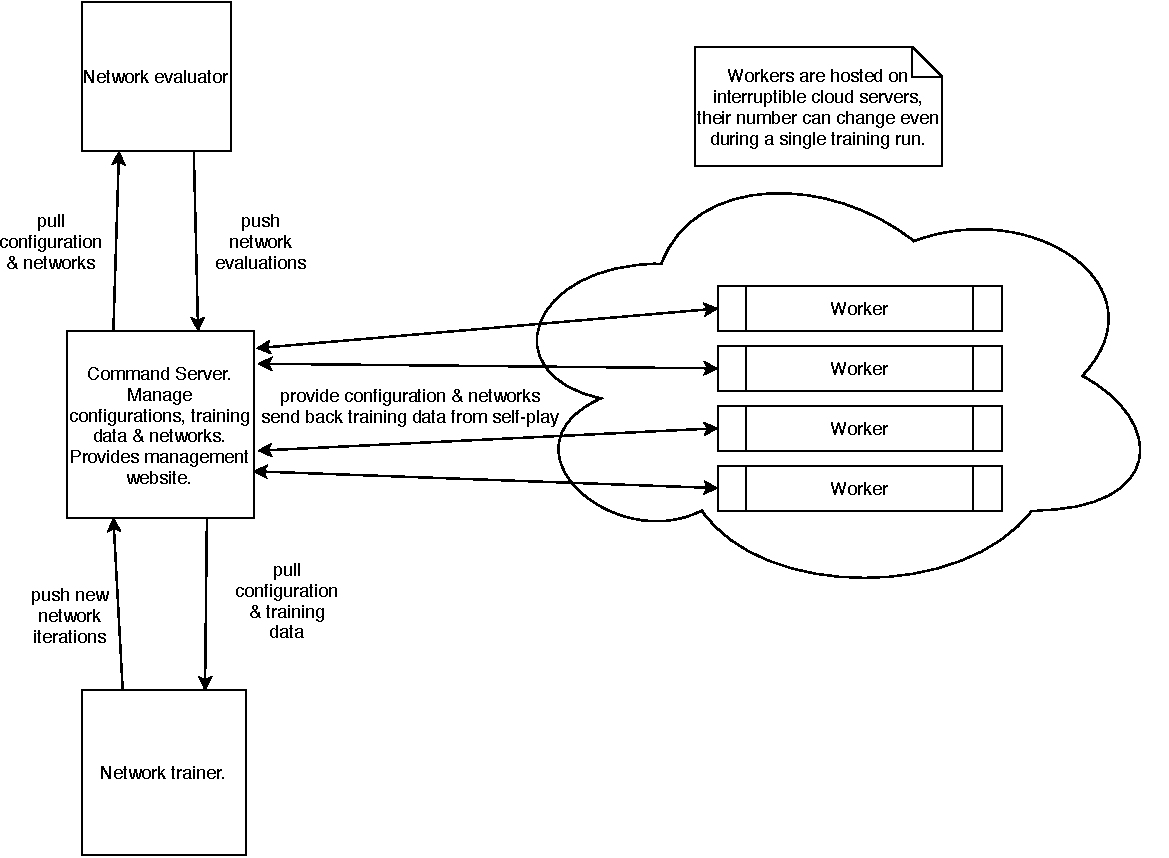
\includegraphics[clip,width=\columnwidth]{x0_framework_overview}
\caption{An overview of the distributed setup for AlphaZero experimentation. A central command server is managing all data and configurations, GPU intensive tasks, such as network evaluation, network training and especially self-play are handled on machines talking to this central server.}
\label{fig:x0_framework_overview}
\end{figure}

All code is available on github\footnote{\url{https://github.com/ColaColin/MasterThesis}}. The repository documents all configuration files used for every experiment mentioned in this thesis and 
for the sake of reproducibility the commit SHA is recorded as well, allowing to reset the code to the exact form it had when a specific experiment was run.

The framework base implementation of AlphaZero uses a different network target for game results, which encodes a dedicated value for a draw. This means for a two player game the possible outcomes are the win of either player, or a draw.
This differs from the original implementation which used a single output with values between zero and one.
There might be a slight change in learning efficiency from this, but the main reasons for it were of technical nature in the context of the abstraction-driven framework and no further research has been done on the difference between these two ways of implementing the value target.

The experiments are split into multiple parts:
\begin{enumerate}
 \item Establish a baseline with a base implementation very close to raw AlphaZero
 \item Implement some known extensions to AlphaZero.
 \item Evaluate proposed ideas one by one.
\end{enumerate}

\subsection{Network architecture}

The network used in all experiments is a minimal modification of the original network used in the AlphaZero work by DeepMind. Modifications are made in the output of the win probabilities, as the original work did not explicitly predict draw chances. Additionally the 
input encoding was adapted for Connect 4.

Position encodings are relative to the player currently making a turn. This includes the input, as well as the output encoding the win chances for the players.
The input encoding converts the $7\times6$ board into a tensor of $1\times7\times6$. Empty fields are encoded as a $3$, the player currently making a move is a $1$, the other player is represented by a $2$. $0$ is not used, as all convolutions 
in the network use padding with $0$, such that all convolutions keep working on a field of size $7\times6$. $0$ thus exclusively represents the edge of the board and the network can learn this.
For the output the move policy is encoded by a flat vector of $7$ values, activated with SoftMax, forming a probability distribution. The win probabilities are encoded as a vector of $3$ values, activated with SoftMax. The first represents the chance of a draw, the second the chance of the
current player winning and the last the chance of the other player winning. The network is shown in Figure \ref{fig:blocks_network}.

The used loss function is the sum of the negative log likelihood of the move policy and the win predictions with the win prediction loss weighted at $0.01$. 


\begin{table} [H]
 \centering
  \begin{tabular}{c | c }
   Description & Network structure \\
   \hline
   \hline
   Initial block & $\begin{pmatrix} 3 \times 3 \times 64 \\ BatchNorm \\ ReLU \end{pmatrix}$ \\
   \hline
   Adapter convolution & $1 \times 1 \times 128$ \\
   \hline
   Residual block, repeated $n$ times & $\begin{pmatrix} 3 \times 3 \times 128 \\ BatchNorm \\ ReLU \\ 3 \times 3 \times 128 \\ BatchNorm \\ Addition \\ ReLU \end{pmatrix}$ \\
   \hline 
   Move policy output & $\begin{pmatrix} 3 \times 3 \times 32 \\ FC: 7 \\ SoftMax \end{pmatrix}$ \\
   \hline
   Win prediction output & $\begin{pmatrix} 3 \times 3 \times 32 \\ FC: 3 \\ SoftMax \end{pmatrix}$
  \end{tabular}
  \caption{Structure of the used network in this work, a smaller and slightly modified version of the original AlphaZero network used by DeepMind \cite{silver2018general}.
  $x \times y \times z$ describes a convolution with kernel size $x \times y$ and $z$ filters. $FC: x$ describes a fully connected layer with $x$ neurons. $Addition$ describes the addition with the input of the residual block the addition is a part of, forming the residual structure of the block.
  The move policy output and the win prediction output both are connected 
  to the output of the last residual block. Residual blocks make up the bulk of the network. In most of this thesis $5$ blocks are used.}
  \label{fig:blocks_network}
\end{table}

\subsection{Testing on Connect 4}

To reduce costs of experiments the game Connect 4 is used. Unlike Go, Connect 4 is a game with a known solution, as it is a solved game for which strong solvers are available \cite{trompsolved, pascalsolver, pascalsolvergithub}, 
i.e. for any given position the solver can quickly find the most optimal move to play.

This makes it possible to evaluate the playing strength of AlphaZero as a measure of accuracy against the strong solver on a dataset of test positions.
It also allows to run supervised training of the used network on a dataset of games played by the solver, establishing a maximum performance possible by the network.

\subsubsection{Generating Connect 4 datasets}
\label{s:generate_dataset}


The generation of the database to be used as a testing set for the learning process is an important step that determines how comparable results are to previous work. 

There is one previous work \cite{oracledevs}[OracleDevs et al.] which published results on Connect 4 using AlphaZero. They claim to reach $97\%$ to $99\%$ accuracy.

Experiments with various datasets have made clear that results can vary wildly between $90\%$ and the claimed $97\%$, depending on the dataset configuration.

One important decision is on what is considered a correct move in a given situation. In Connect 4 there are many positions where the player has multiple ways to force a win, but some may lead to a longer game before the win is forced.
\cite{oracledevs} defines here \emph{strong} and \emph{weak} testsets: 

A \emph{strong} testset only considers a move correct if it yields the fastest win or the slowest loss. 

A \emph{weak} testset only cares about the move producing the same result 
as the best move, no matter how much longer the win will take or how much faster the loss will occur.

They report $97\%$ accuracy on strong datasets and $99\%$ on weak datasets.

Additional important decisions made in the dataset creation which are not talked about in detail by previous work are:

\begin{enumerate}
 \item How to play the games exactly? Only perfect moves or make some mistakes?
 \item Should duplicate positions be filtered out?
 \item Should trivial positions, i.e. positions that have no wrong answer, be filtered out?
\end{enumerate}

Experiments with various options showed that especially the question of how games are played can substantially influence the final accuracy values. A dataset generated by playing $50\%$ random moves and $50\%$ perfect moves, found
by a solver \cite{pascalsolver, pascalsolvergithub}, is substantially harder than a dataset created using
$90\%$ perfect and only $10\%$ random moves. This appears to be mainly a result of the distribution of game length, shown in Figure \ref{fig:dataset_hist}, as less random moves produce a dataset with more positions in the late game, while more random moves cause more positions to be in the early game.
Making the right move in turn $10$ is a lot harder than in turn $30$, as the remaining game tree is much larger in the earlier phase of the game. Using supervised training, described in section \ref{sec:supervised}, the harder dataset can only reach about $92.6\%$ accuracy whereas the easier dataset
can reach $96.97\%$, very close to the $97\%$ claimed by previous work. 

\begin{figure}[H]
\centering
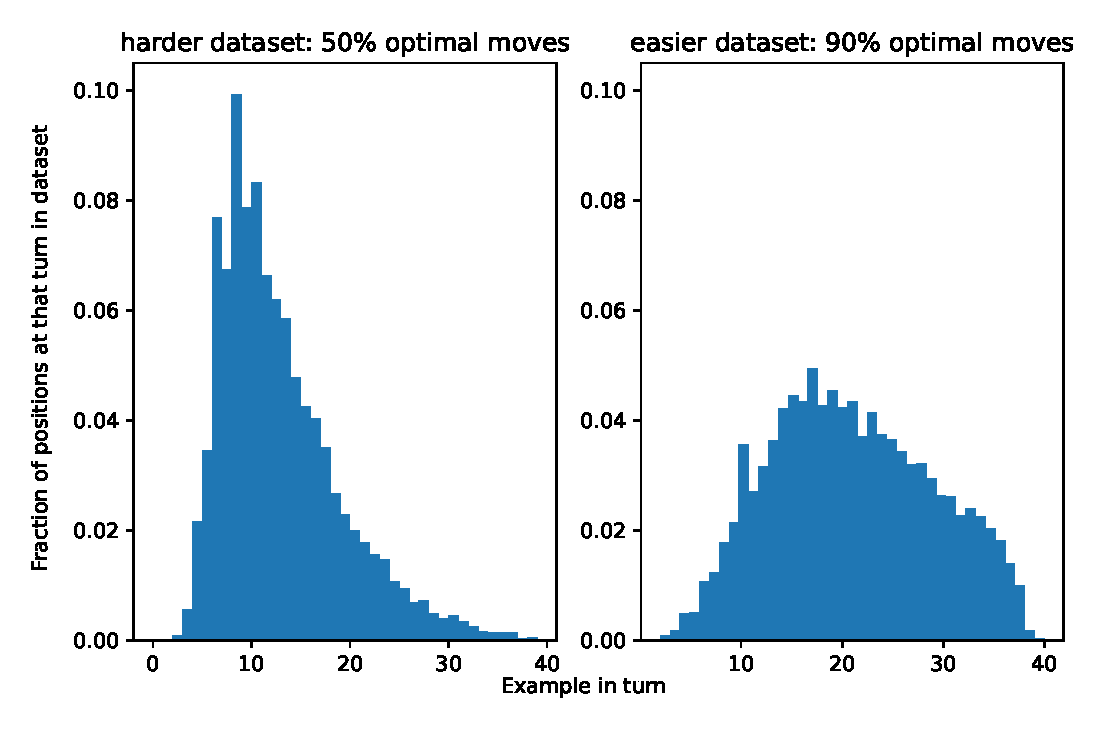
\includegraphics[clip,width=\columnwidth]{dataset_hist}
\caption{Different ways of generating the dataset can cause a substantially different distribution of examples.}
\label{fig:dataset_hist}
\end{figure}



For most of the following experiments the harder dataset, playing $50\%$ random moves, was used. If a dataset is specified, they will be referred to as the easy and the hard dataset from here on.
For all other options the hardest possible settings were used to create a maximally challenging dataset:
No duplicates, without trivial positions and only the strongest possible moves are accepted as correct.

The average number of correct moves per position can be used as a metric to determine how challenging a dataset is. The generated maximally hard dataset, $50\%$ random moves, has on average $1.8$ correct moves per position.
The generated easier dataset, playing $10\%$ random moves, has $1.95$ correct moves per position.

In contrast \cite{oracledevs}[OracleDevs et al.] report $4.07$ correct moves per position in their weak dataset and $2.16$ correct moves per position in their strong dataset, indicating they made choices which noticeably reduced the challenge their dataset posed, 
possibly explaining differences in accuracy values between this work and theirs.

\subsection{Evaluation of training costs}

The goal of this thesis is to identify ways to reduce the substantial costs of training using AlphaZero. The majority of GPU capcacity is spent on self-playing games to be used as training material for the neural network.
In all experiments neural network training is done on a single GPU, newly produced networks are evaluated on another single GPU and self-play workers are run on a p2p cloud service\footnote{\url{https://vast.ai}} using up to 20 GPUs of various types to complete full training runs
for Connect 4 in $2$ to $6$ hours, depending on the number of self-play workers.

This huge imbalance between training hardware and self-play hardware can be seen in related work as well, e.g. \cite{AlphaZero}[Silver et. al.] used $5000$ first-generation TPUs for self-play and $16$ second-generation TPUs 
to learn play Chess on super-human, and potentially even super-classical-engine, level within hours. Similarly \cite{wu2019accelerating}[David J. Wu] used up to $24$ V100 GPUs to produce self-play training examples to feed a single V100 GPU training data for neural network training to play Go.

The bulk of the training cost consequently lies in the self-play workers. For all experiments in this thesis this fact will be used to simplify the training cost measurement by ignoring the costs of the network training. Instead only the cost of self-playing workers is measured.

Since the main source of computational resources for self-play is a p2p cloud service which provides unreliable but cheap GPU time there is no constant number of GPU workers between experiments or the number of self-play workers even changes during training.

After an experiment is completed a benchmarking program is run on a reference machine using the produced networks and measures how much time is needed on average 
to play a single move. This value is then used to estimate the cost of the actual number of moves that were played by the self-play workers during the experiments.

This reference machine uses a single Nvidia RTX 2070S, which is saturated to $100\%$ load by the benchmark. Thus all self-play cost of experiments is stated as estimated self-play time on that machine and bottlenecked by GPU capcacity on it.

\subsection{Supervised training}\label{sec:supervised}

To provide guidance on how good the results of AlphaZero are, supervised training of the networks is used to establish the maximum possible performance of the network.
For this a dataset of 1 million Connect 4 positions, generated using $50\%$ random moves as outlined in section \ref{s:generate_dataset}, is employed. Two versions of the dataset are generated, in version 1, all positions of played games are used as training data.
In version 2 of the dataset, only a single position is randomly picked from each played game, increasing the number of distinct games played to generate the dataset substantially.

For both versions of the dataset, $800000$ examples were used as training data, $100000$ examples were used as validation data and the remaining $100000$ examples were used as test data.
Training started with a learning rate of $0.2$ and was reduced by a factor of $10$ after $8$ epochs of no accuracy improvements on the validation data. The supervised training stops after $12$ epochs with no improvements on the validation accuracy.

Various network sizes are evaluated. Mean results of five runs for each network are shown in table \ref{t:supervised_results}. One additional set of five $5$-blocks network were trained using the easier $10\%$ random moves dataset, they reached a mean supervised accuracy
of $96.94\%$ on move prediction and $84.75\%$ on win prediction, highlighting the big difference in achieved accuracy between the harder and the easier dataset.

\begin{table} [H]
 \centering
  \begin{tabular}{ l | c c c c c }
  Network & parameters & moves $\%$ v1 & wins $\%$ v1 & moves $\%$ v2 & wins $\%$ v2 \\
  \hline
  5-blocks & $1574730$ & $91.63\%$ & $77.47\%$ & $92.44\%$ & $79.23\%$ \\
  10-blocks & $3053130$ & $92.37\%$ & $77.87\%$ & $93.00\%$ & $79.67\%$ \\
  20-blocks & $6009930$ & $92.68\%$ & $78.23\%$ & $93.49\%$ & $79.93\%$ \\
  \end{tabular}
  \caption{Results of supervised training. Accuracy compared to a connect 4 solver.}
  \label{t:supervised_results}
\end{table}


What surprises of these results is the quite low accuracy on the prediction of the winner of a match, as AlphaZero training runs achieve values close to $90\%$ win-prediction accuracy.
This hints at some problem with the supervised training data.

To rule out overfitting on the dataset, another dataset, using the $10\%$ random moves, with 10 million positions taken from 10 million games was generated. This dataset achieved a move prediction accuracy with the $5$-block network 
of $97\%$, but the win-prediction still stayed below the accuracy reached in AlphaZero training runs, that played less than 10 million games overall.
Given that the used $5$ block network only has about $1.5$ million parameters, overfitting on a dataset of $10$ million examples seems unlikely.

Since overfitting is ruled out as a cause, it seems likely the issue is that a dataset generated from games with a certain fraction of random-moves does not provide optimal training quality to predict the outcome of perfect-play games, which causes the low win-prediction accuracy.
Games played on the best level AlphaZero can accomplish are not perfect, but mistakes made are much different from just playing random moves. This seems to be mirrored in the win prediction accuracy.


\subsection{Baseline}

Various baselines need to be established to compare novel proposals against. Supervised training of the used networks allows to explore the maximum possible performance, a plain AlphaZero baseline shows how the original algorithm performed, while a baseline
of AlphaZero extended with a set of previously known improvements shows the progress made since the original algorithm was published.

For all experiments, unless noted otherwise, the MCTS uses trees with $343$ nodes, which was picked as it represents the number of nodes to fully search $3$ moves ahead in Connect 4: $7^3$,
networks will be trained in iterations of $300000$ produced examples. Every network is evaluated on the test set for accuracy compared with the Connect 4 solver.
Network training happens using SGD with momentum of $0.9$, weight decay of $0.0001$. The learning rate starts at $0.2$, is dropped to $0.02$ in iteration $7$ and $0.002$ at iteration $14$. 
Gradient clipping at a magnitude of $1$ is used to stabilize training at the maximum learning rate of $0.2$.
A training window of $2$ million positions is used.


Based on the results of the supervised training and under consideration of the training costs all experiments are done with the $5$ block network, which has about $1.5$ million parameters. A larger network might reach slightly better results,
but the goal of this thesis is to look for efficiency gains, not maximum final performance. Therefore the smaller network is used to allow for faster experimentation.

\subsubsection{Hyperparameter search}

The AlphaZero algorithm requires some important hyperparameter values, which can make a large difference on the learning efficiency. 

To establish a baseline with sensible hyperparameter a Bayesian hyperparameter optimization with $65$ search steps was used.
In each search step the AlphaZero algorithm was run on a single machine, which alternated between self-play and training. The Bayesian optimization was tasked with optimizing the accuracy after two hours of real time. 

To yield meaningful results after just two hours on a single GPU,
the size of iterations were chosen in such a way to make faster progress, at the cost of the quality of the final results, i.e. less games were played per network trained and the MCTS-trees were smaller when playing games. Thus the accuracy values reached were rather low, around $80\%$,
but still allowed for a relatively quick comparison between different hyperparameters. 

After this initial search, three sets of hyperparameters were selected and evaluated with full experimental runs to maximum accuracy to pick the best hyperparameters for the following work.

The hyperparameters optimized for are listed in table \ref{t:hyperparameters}. A preliminary run of hyperparameter optimization was used to inform the decision to optimize these parameters in particular.

\begin{table}[H]
  \centering
    \begin{tabularx}{\textwidth}{lX}
    \toprule
    Parameter     & Description \\
    \midrule
    cpuct          & The $C_{puct}$ constant of AlphaZero, see equation \ref{eq:alpha_zero_u} on page \pageref{eq:alpha_zero_u}. \\
    \hline
    fpu          & First play urgency. The value of a move which has not been played yet at all during MCTS, it has some control over the balance between exploration and exploitation as well. \\
    \hline
    alphaBase          & Determines the value of $\alpha$, which is a constant used in AlphaZero to control explorative noise. alphaBase is an extension to adapt to the fact that the raw $\alpha$ value highly depends on the number of legal moves a game has on average.
      alphaBase is used to calculate the value of $\alpha$ depending on the number of legal moves: $\alpha = \frac{alphaBase}{n}$ where $n$ is the number of legal moves. 
      In the context of Connect 4 with a 7x6 board alphaBase thus needs to be divided by at most $7$ to determine the corresponding $\alpha$ value in the context of the original implementation. \\
      \hline 
    drawValue & Determines the value of a draw when calculating the value of a position in a MCTS node. This parameter does exist because of the different way chosen to implement the network value output, which produces
  an output indicating the likelihood of a draw. To estimate the value of a position the formula $W + D*drawValue$ is used, where $W$ is the network estimation of a win and $D$ the estimation for a draw. A high value thus makes draws
  as desirable as wins, a low value as undesirable as losses.\\
    \bottomrule
    \end{tabularx}%
  \label{tab:addlabel}%
  \caption{Hyperparameters searched}
  \label{t:hyperparameters}
\end{table}

The hyperparameters chosen for further investigation in full experimental runs are shown in table \ref{t:hyper_search_results}. Hyperopt1 and hyperopt2 were the two best sets found by the hyperparameter search. prevWork is based on results of previous work.

\begin{table} [H]
 \centering
  \begin{tabular}{ l | c c c c }
  Name & cpuct & fpu & alphaBase & drawValue \\
  \hline
  hyperopt1 & $0.9267$ & $0.91$ & $12.5$ & $0.4815$ \\
  hyperopt2 & $1.545$ & $0.8545$ & $20.38$ & $0.6913$ \\
  prevWork & $4$ & $0$ & $7$ & $0.5$ \\
  \end{tabular}
  \caption{Hyperparameter sets selected for further investigation.}
  \label{t:hyper_search_results}
\end{table}

Full training runs are done $5$ times for every of the hyperparameter sets under investigation. In every run the training is stopped once the MCTS accuracy has not improved for $10$ iterations.
The $5$ runs are used to calculate a mean, which is used to compare the different runs against each other.

\begin{figure}[H]
\centering
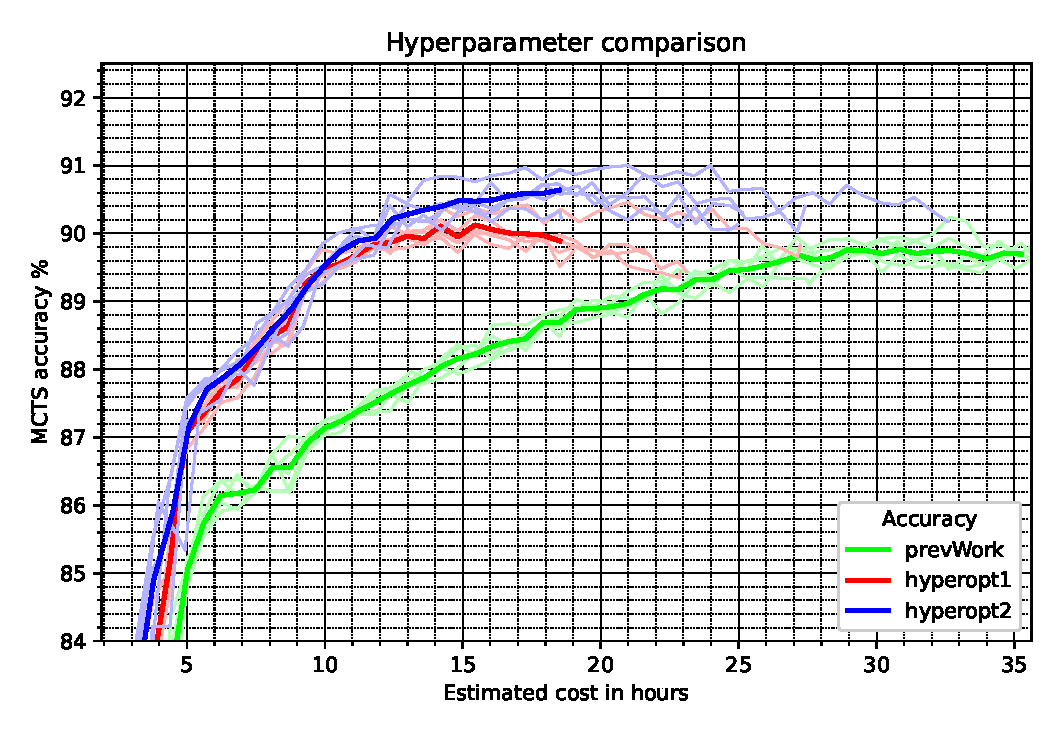
\includegraphics[clip,width=\columnwidth]{hyper_compare}
\caption{Results of the runs to determine a good hyperparameter set. Mean is only calculated until the first of the single runs stops showing improvements.}
\label{fig:hyper_compare_results}
\end{figure}


It can be seen that the results of the parameters taken from previous works fall substantially behind the values found via Bayesian optimization. This is likely due to the fact that previous work was on other games, 
using different implementation details, such as different tree sizes, iteration sizes, network sizes or other differences.

The hyperparameter set hyperopt2 is used for all further experiments, its performance forms the baseline on which improvements are investigated.

\subsection{Extended Baseline} \label{s:exexp}

As outlined in section \ref{s:prev_extensions} on page \pageref{s:prev_extensions}, much work has been done to propose various ways of improving learning efficiency of AlphaZero. 

The differentiation between the AlphaZero baseline and the extended AlphaZero baseline is important to verify proposed improvements are cumulative with already known ways to improve AlphaZero.


\subsubsection{Remove duplicate positions}

Especially for games such as Connect 4 there are a lot of duplicate positions in the training data. Depending on various exploration hyperparameters and training progress, this causes between $30\%$ and $80\%$ duplicate positions to be reached.
The neural network training thus is provided with a large set of duplicate input values, which will have conflicting target values to be learned. Additionally positions early in the game will be overrepresented in the training data, as they make up the vast majority of
duplicate positions.

In the context of Connect 4 \cite{oracledevs6}[OracleDevs et al.] propose to merge duplicate positions to counteract this.

This thesis implements this by acting in the training worker, only new positions are added to the pool of training examples, previously known positions instead update the target value
for that position.

For this purpose a record of all previously known positions is kept in a hash map.
Every time a duplicate is produced by a self-play worker and send to the training worker, the training worker will merge the new target values with the old target values of the duplicate using a weight
$w_{\text{duplicate}}$: $$\text{target}_{\text{new}} = \text{target}_{\text{old}} * (1 - w_{\text{duplicate}}) + \text{target}_{\text{duplicate}} * w_{\text{duplicate}}$$

The higher $w_{\text{duplicate}}$, the less importance is given to previous targets for a position. At the maximum value of $1$,
targets are completely replaced whenever a new report on a position comes in.

The values $0.2$, $0.5$ and $0.8$ are tested in single runs and compared against the baseline to evaluate how promising this approach is. Figure \ref{fig:dedupe_cmp} shows the results. 

A noticeable improvement can be seen. $0.8$ appears to outperform the baseline the most and is chosen to be part of the extended baseline configuration.

To keep the size of iterations consistent with previous experiments, network iterations are now reduced to once every $180000$ new examples. With the typical rate of duplicates during a baseline run, this comes out at about $300000$ positions played per iteration, at least in the first part
of the training. The more duplicates are produced during play, the longer iterations become in real time, as less and less new examples are generated.
The training window stays at $2$ million positions, which however now all will be distinct from each other.

\begin{figure}[H]
\centering
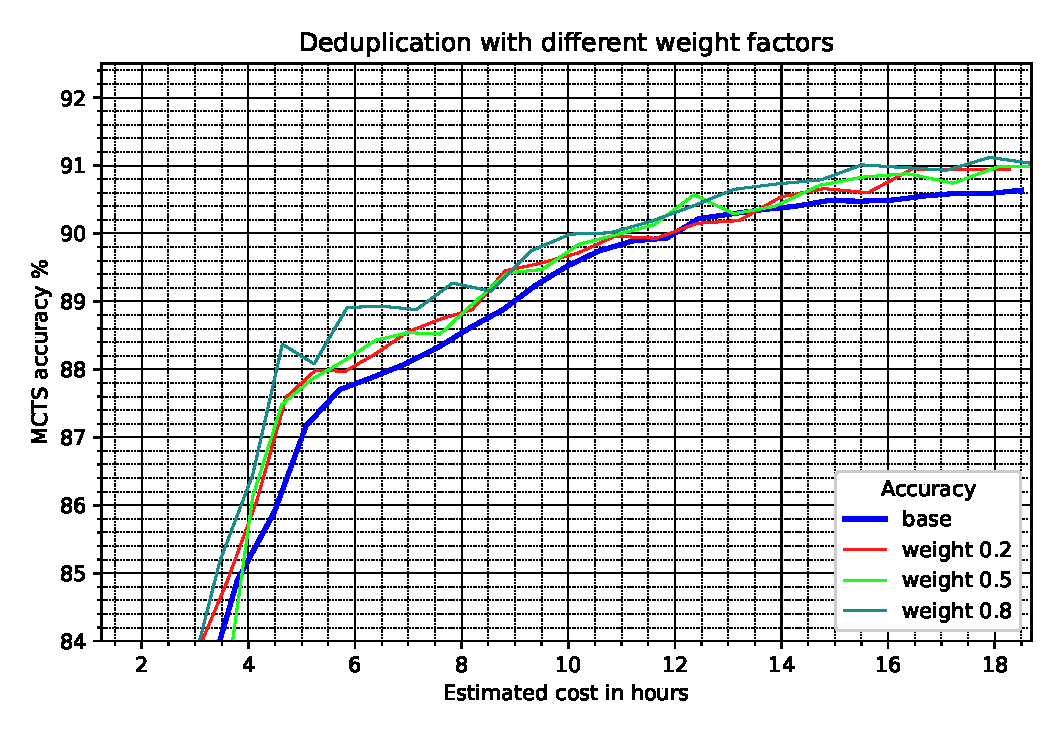
\includegraphics[clip,width=\columnwidth]{dedupe}
\caption{Comparison of different choices for $w_{\text{duplicate}}$. $0.8$ is chosen for all further experiments.}
\label{fig:dedupe_cmp}
\end{figure}


\subsubsection{Cyclic learning rate}

Cyclical learning rates are a proposal by \cite{smith2017cyclical}[Smith et al.] to speed up general neural network training. \cite{oracledevs6}[OracleDevs et al.] claim some improvement using them in the context of AlphaZero.

Based on these claims cyclic learning rates and cyclic momentum have been implemented for AlphaZero as a potential addition to the extended baseline. The cycles are over single iterations of the network, thus $300000$ examples 
using the baseline or $180000$ new examples using deduplication.


\begin{figure}[H]
\centering
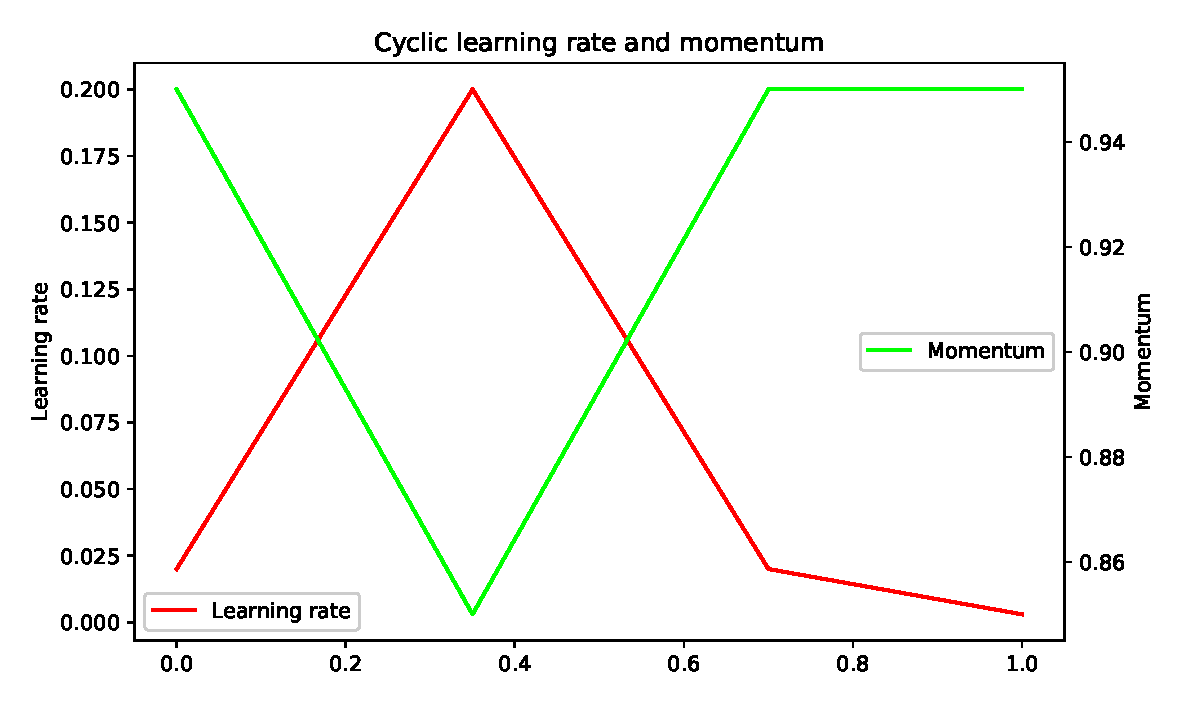
\includegraphics[clip,width=\columnwidth]{cyclic}
\caption{The change of the learning rate and momentum over the training of a new network iteration when using cyclic learning rates.}
\label{fig:cyclic_lr}
\end{figure}

The learning rate starts out at $0.02$, reaches its peak of $0.2$ at $35\%$ of the iteration, then starts to drop back to $0.02$, which is reached by $70\%$ of the iteration, finally the learning rate is dropped down to $0.003$ by the end of the iteration.
Using the same proportions over the iteration, the momentum starts at $0.95$, drops to $0.85$ and then rises back to $0.95$.
The values are informed by previous runs to determine the maximum and minimum useful learning rate, especially the supervised training which reduced the learning rate automatically using early stopping.


These curves can be seen in figure \ref{fig:cyclic_lr}.
Additionally, not shown in the figure, the learning rate is annealed down with a multiplicative factor that drops with the network iterations in a linear fashion. It starts at $1$ in iteration $1$ and reaches $0.4$ in iteration $20$. Beyond iteration $20$ the factor stays at $0.4$.
Thus at iteration $20$ and later, the maximum learning rate is $0.08$.


A single run was done with the baseline configuration, using the described cyclic learning rate and momentum. The results can be seen in figure \ref{fig:cyclic_results}.
Slight improvements were found, especially in the earlier stages of the training. Cyclic learning rate and momentum was added to the extended baseline 
configuration. 


\begin{figure}[H]
\centering
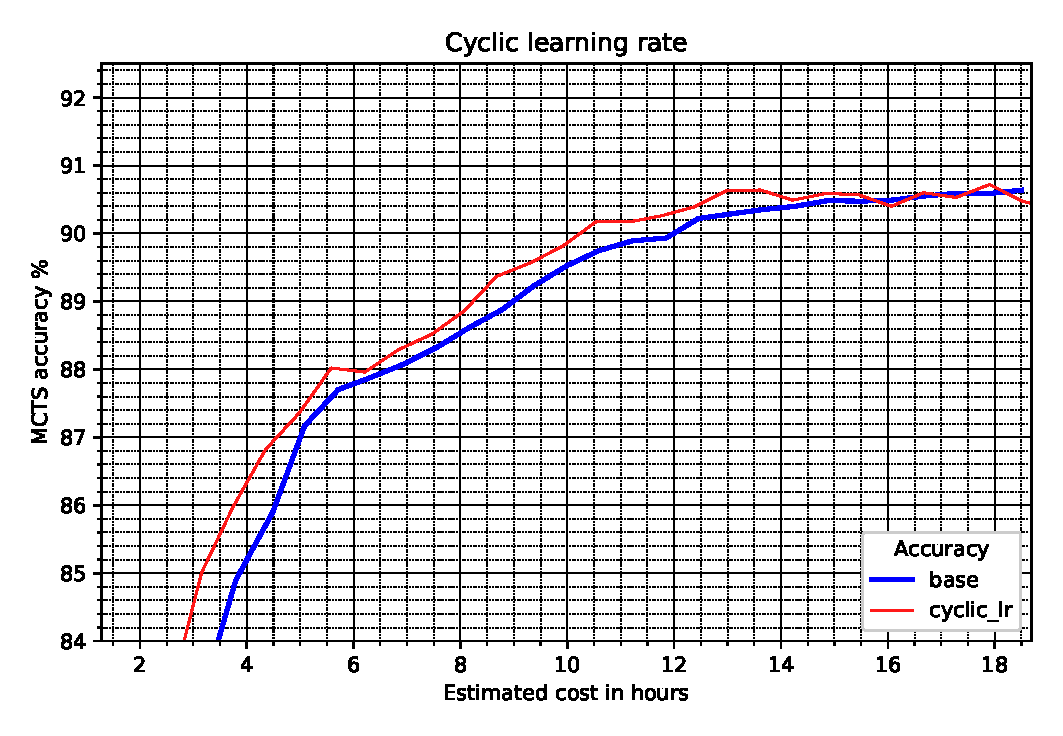
\includegraphics[clip,width=\columnwidth]{cyclic_results}
\caption{Comparison of the usage of cyclic learning rates and momentum with the baseline.}
\label{fig:cyclic_results}
\end{figure}



\subsubsection{Improved training window}

\cite{oracledevs6}[OracleDevs et al.] noticed that a jump down in the training error can be observed in the first iteration that pushes the examples of the very start of the training out of the training window. It stands to 
reason that these are especially bad training examples, as the network at that point would be very close to random play. This motives to let the training window start out small and grow over a number of iterations. This way the 
training examples of early iterations are removed from the training data more quickly. This is called a slow training window.

For this thesis a slow training window is implemented, it starts with a size of $500000$ examples, which grows between iteration $5$ and $12$ up to the maximum size of $2$ million examples. This causes early examples to be removed by iteration $3$.

A single run is done to evaluate the effects of this modification, the results are seen in figure \ref{fig:slow_window_results}. 

\begin{figure}[H]
\centering
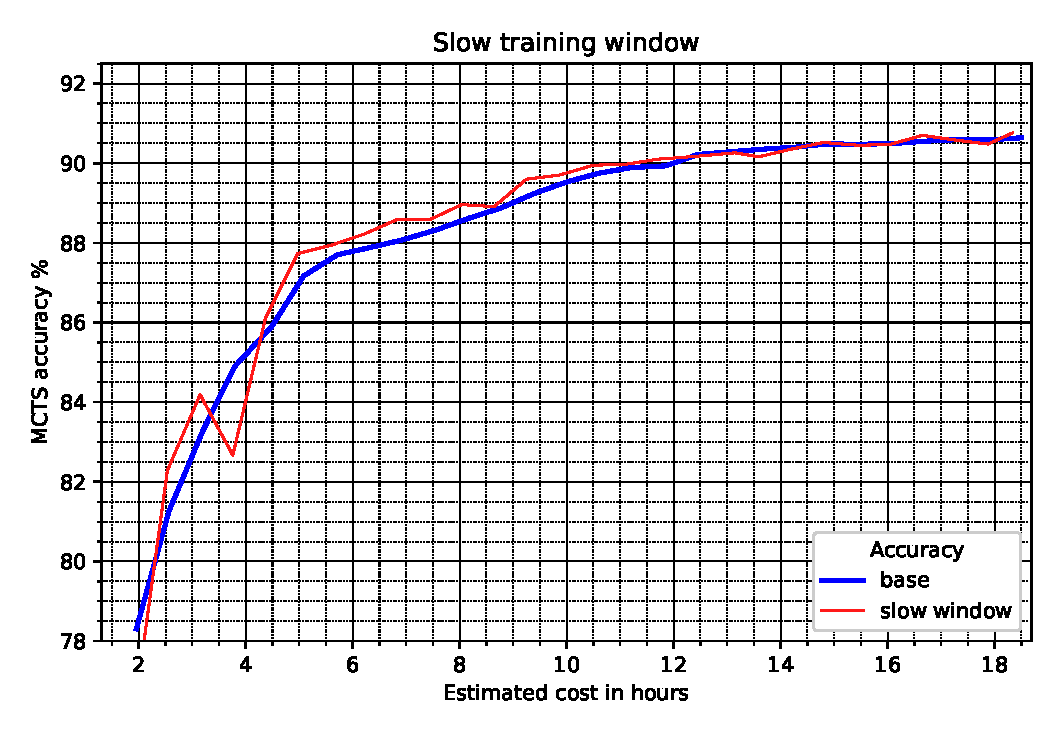
\includegraphics[clip,width=\columnwidth]{slow_window}
\caption{Comparison of the usage of a slow training window with the baseline.}
\label{fig:slow_window_results}
\end{figure}

The slow window is added to the extended baseline, since it does not appear to hurt and it follows a sound idea. To accommodate the fact that the extended baseline uses a training window without duplicate positions the parameters are modified
to grow from iteration $5$ to $15$, since the number of new examples per iteration is lower.

\subsubsection{Playout Caps}

Playout Caps \cite{wu2019accelerating}[Wu et. al.] implement the idea to play, at random, a substantial fraction of all moves with a substantially reduced number of nodes in the MCTS and only record moves played with the full number of nodes used.
This means a lot more games are played at a marginal additional cost. Since the moves played with a less deep MCTS are not recorded, the training data does not reduce in quality, but more distinct game results are collected.
This can help provide better quality data for the value target of the network, which predicts the winner of games. Wu et. al. claim $27\%$ improvement in Go, which is notorious for especially long games.

Playout Caps have been implemented for this Thsis and have been evaluated on Connect 4. For $75\%$ of the moves played the number of MCTS nodes was reduced to $30$, only the moves played with the standard $350$ nodes in the other $25\%$ were recorded as training data.
Results of a test run can be seen in figure \ref{fig:playout_caps}.

\begin{figure}[H]
\centering
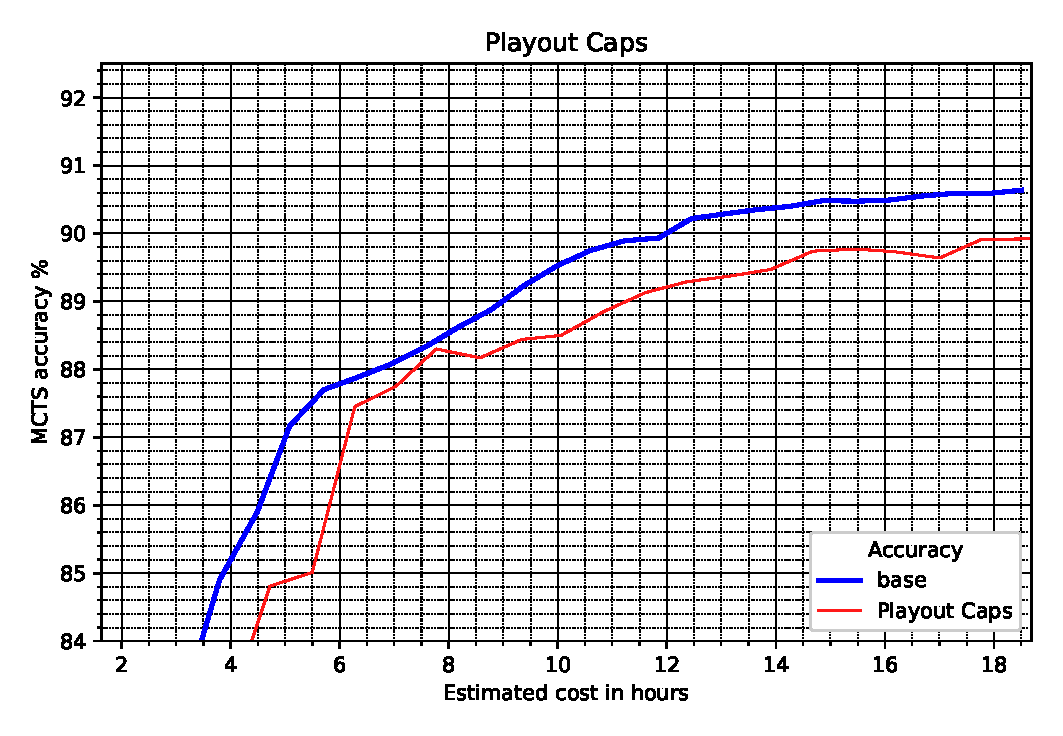
\includegraphics[clip,width=\columnwidth]{playout_caps}
\caption{Results of implementing Playout Caps on Connect 4.}
\label{fig:playout_caps}
\end{figure}

Clearly Playout Caps appear to hurt performance on Connect 4. This likely stems from the fact that an average Connect 4 game tends to take $30$ moves. A game of Go, for which Playout Caps were developed, averages at $211$ moves\footnote{\url{https://homepages.cwi.nl/~aeb/go/misc/gostat.html}}.
This means the AlphaZero learning to play Go will be a lot more pressed for more game result training data, than AlphaZero learning to play Connect 4.

Playout Caps were not made part of the extended baseline.

\subsubsection{Predicting the opponent's reply.}

\cite{wu2019accelerating}[Wu et. al.] shows that predicting the opponent's reply after the current position produces a ''modest but clear beneft``.
Specifically they propose to add a term to the loss function to regularize training:

\begin{equation}
 -w_{\text{opp}} \sum\limits_{m \in \text{moves}} \pi_{\text{opp}}(m) \log(\hat{\pi}_{\text{opp}}(m)) \label{eq:opp_reply}
\end{equation}

where $\pi_{\text{opp}}$ is the policy target for the turn after the current turn, $\hat{\pi}_{\text{opp}}$ is the network's prediction of $\pi_{\text{opp}}$ and $w_{\text{opp}}$ is a weight for the loss term. In the experiments with Connect 4, $0.35$ is used.

Figure \ref{fig:predict_reply} shows the results of testing this on Connect 4. There appears to be a small advantage for some parts of the run, therefore this was made part of the extended baseline.

\begin{figure}[H]
\centering
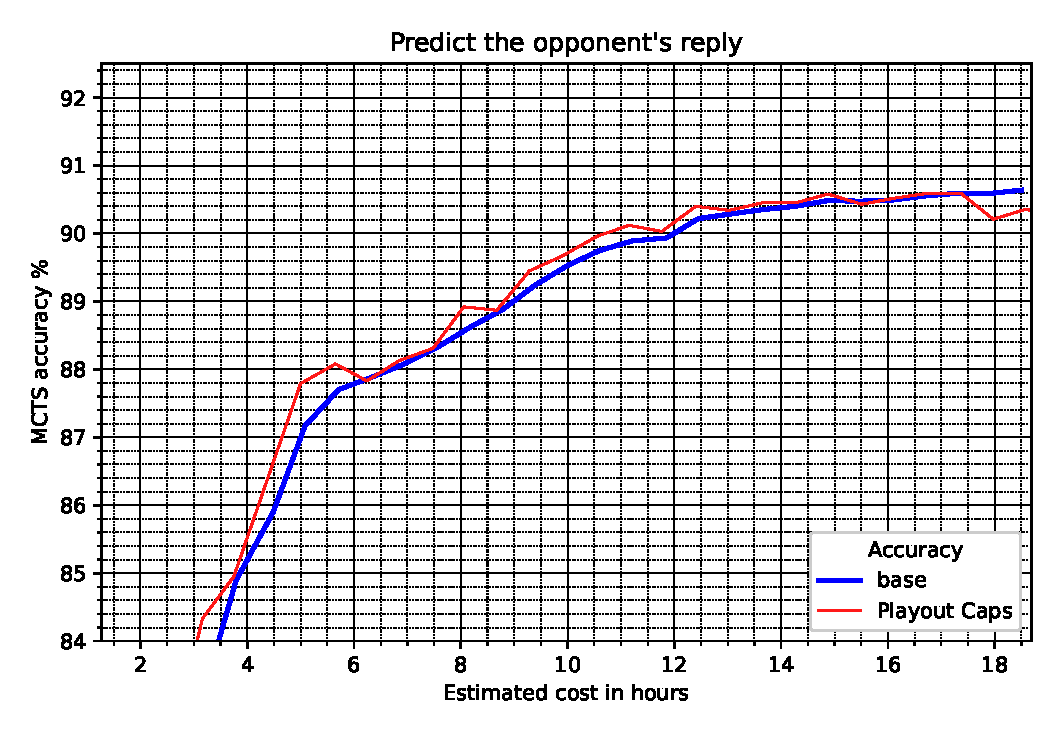
\includegraphics[clip,width=\columnwidth]{predict_reply}
\caption{Results of implementing the prediction of the opponent's reply.}
\label{fig:predict_reply}
\end{figure}


\subsubsection{Improving the network structure}

The Leela Chess Zero project \cite{leela0sq} proposes to use Squeeze and Excitation elements in the network.
These are a general development of deep neural networks  \cite{hu2018squeeze}, which have been shown to improve learning efficiency at a small additional cost.

The network described in Table \ref{fig:blocks_network} on page \pageref{fig:blocks_network} was modified for this, the resulting network is shown in table \ref{fig:sq_blocks_network}.

\begin{table} [H]
 \centering
  \begin{tabular}{c | c }
   Description & Network structure \\
   \hline
   \hline
   Initial block & $\begin{pmatrix} 3 \times 3 \times 64 \\ BatchNorm \\ ReLU \end{pmatrix}$ \\
   \hline
   Adapter convolution & $1 \times 1 \times 128$ \\
   \hline
   SQ residual block, repeated $n$ times & $\begin{pmatrix} 3 \times 3 \times 128 \\ BatchNorm \\ ReLU \\ 3 \times 3 \times 128 \\ BatchNorm \\ AVG Pooling \\ FCnb: 8 \\ ReLU \\ FCnb: 128 \\ Sigmoid \\ Addition \\ ReLU \end{pmatrix}$ \\
   \hline 
   Move policy output & $\begin{pmatrix} 3 \times 3 \times 32 \\ FC: 7 \\ SoftMax \end{pmatrix}$ \\
   \hline
   Win prediction output & $\begin{pmatrix} 3 \times 3 \times 32 \\ FC: 3 \\ SoftMax \end{pmatrix}$
  \end{tabular}
  \caption{The modified network using Squeeze and Excitation Residual blocks \cite{hu2018squeeze}.
  Squeeze and Excite modifies the residual blocks to include an average pooling, which averages every feature map to a single scalar value. These scalar values are then processed by fully connected layers without bias, activated by ReLU and Sigmoid.
  $x \times y \times z$ describes a convolution with kernel size $x \times y$ and $z$ filters. $FC: x$ describes a fully connected layer with $x$ neurons. $Addition$ describes the addition with the input of the residual block the addition is a part of, forming the residual structure of the block.
  The move policy output and the win prediction output both are connected 
  to the output of the last residual block. Residual blocks make up the bulk of the network. In most experiments of this thesis $5$ blocks are used.}
  \label{fig:sq_blocks_network}
\end{table}

A result of a test run can be seen in figure \ref{fig:sqnet}. 
It appears there might be some gains early in the training and possibly some small losses later in the training. I have decided to add this modification to the extended baseline, as it does not seem to hurt performance much and 
logically should help, especially given more distinct training data from deduplication.


\begin{figure}[H]
\centering
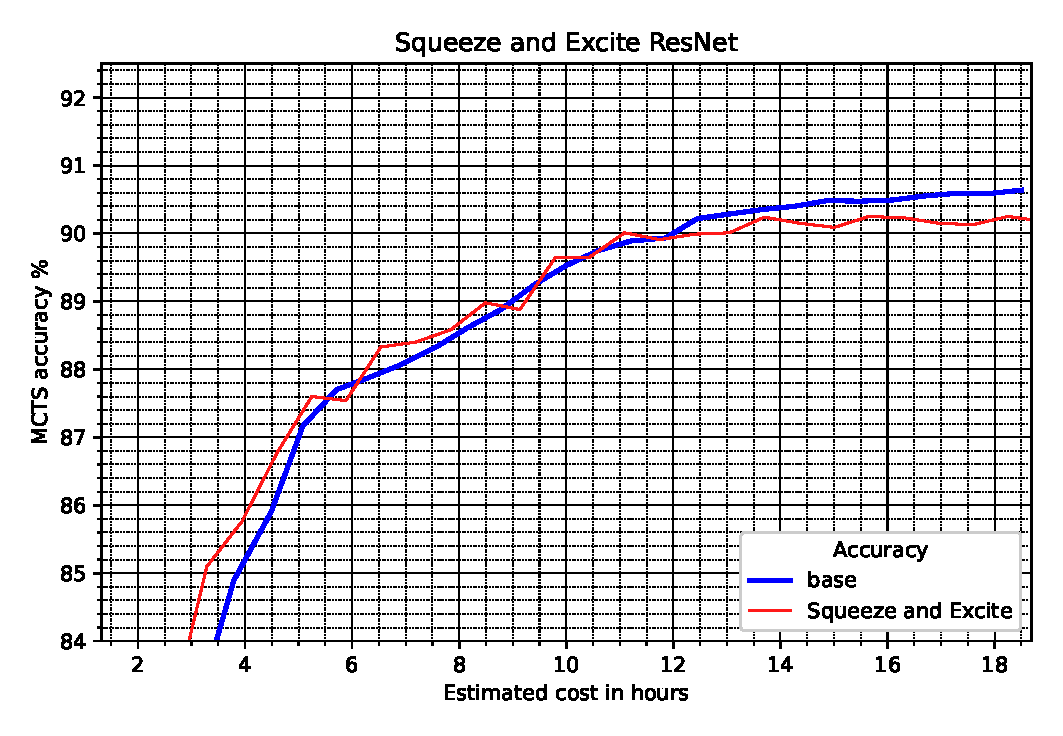
\includegraphics[clip,width=\columnwidth]{sqnet}
\caption{Results of implementing Squeeze and Excitation elements in the network.}
\label{fig:sqnet}
\end{figure}


\subsection{Baseline results}

Combining deduplication, a cyclic learning rate, a slow window, predicting the opponents reply and squeeze-and-excitation elements yields substantial improvements, yielding above $91\%$ final performance in all runs on the hard dataset. The results can be seen in figure \ref{fig:baseline_compare}.
The easy dataset shows the same improved efficiency, further validating the improvements proposed by previous work.
This extended baseline forms the basis of all further experiments, unless stated otherwise all these previous improvements are active.

\begin{figure}[H]
\centering
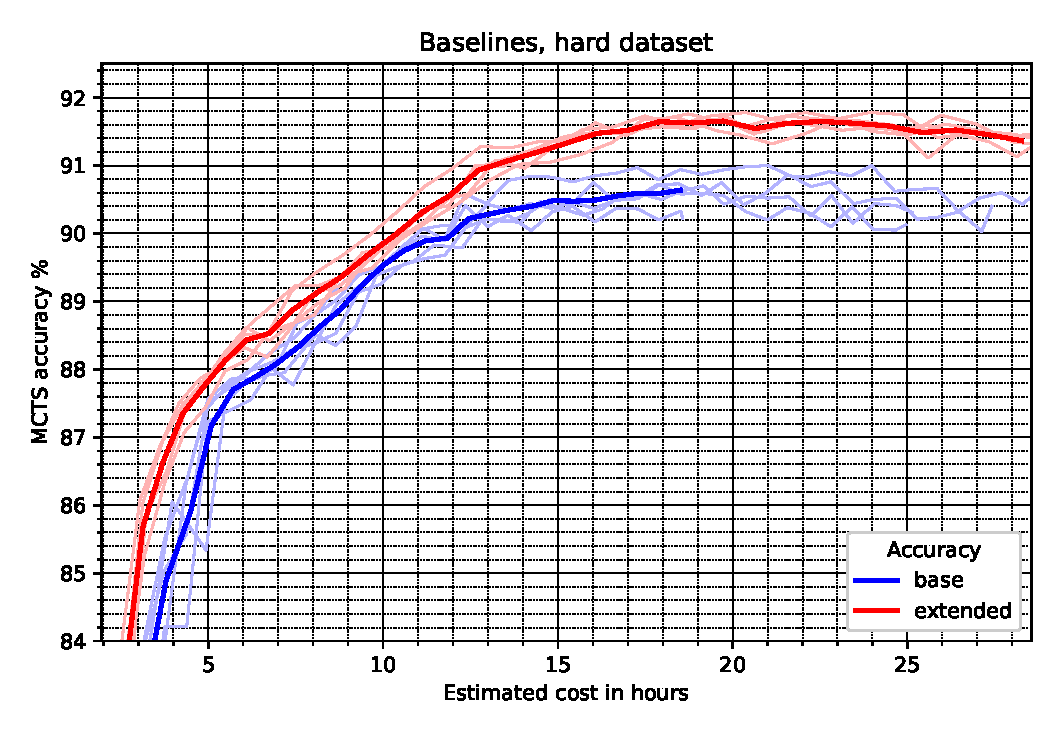
\includegraphics[clip,width=\columnwidth]{baseline_ex}
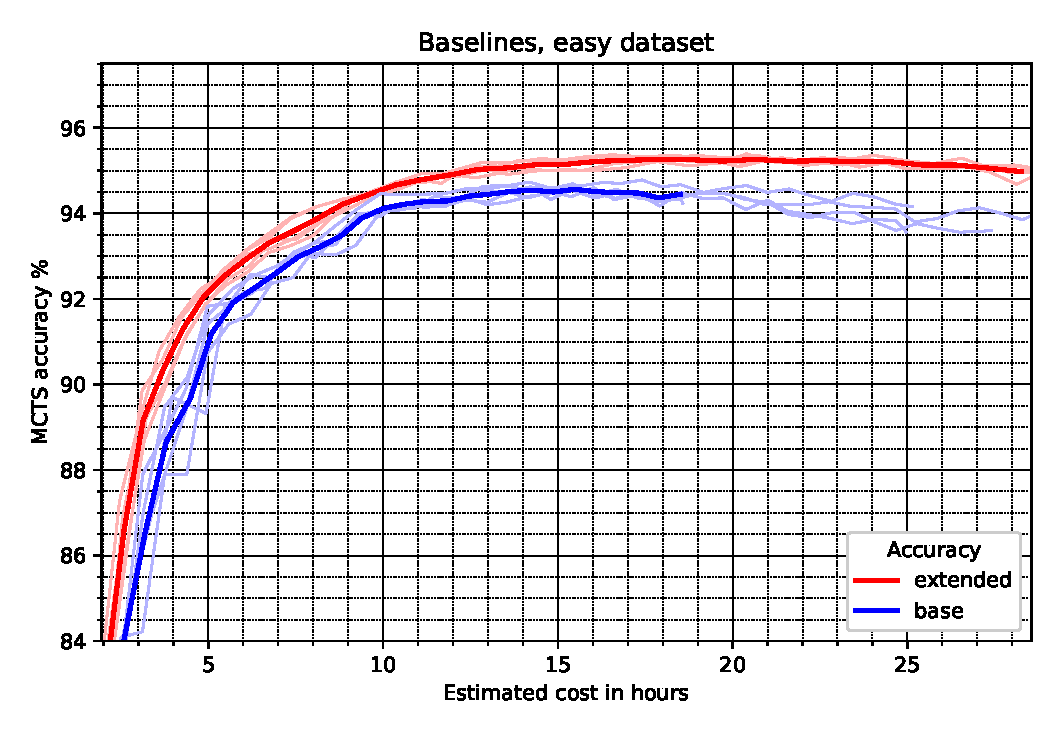
\includegraphics[clip,width=\columnwidth]{baseline_ex_easy_dataset}
\caption{Comparison of the baseline and the extended baseline. Mean is only calculated until the first of the single runs stops showing improvements.}
\label{fig:baseline_compare}
\end{figure}


\section{Investigated novel ideas}\label{s:novel_ideas}

In this section various novel ideas on possible improvements to AlphaZero are investigated experimentally.

\subsection{Using the self-playing phase as an evolutionary process} \label{s:novel_evolution}

There are many hyperparameters involved in AlphaZero which have to be tuned. An important subset of these hyperparameters controls the exact behavior of the MCTS search, for example $C_{puct}$, as discussed in section \ref{s:azalgo}, Equation \ref{eq:alpha_zero_u} on page \pageref{eq:alpha_zero_u}.
A hyperparameter search shows that these MCTS-parameters have a notable impact on how much the MCTS can improve the playing strength of the network alone. Better parameters therefore could translate into faster training progression.

This thesis proposes to use the self-playing phase of AlphaZero to optimize these hyperparameters by designating ''players``, which utilize different hyperparameters and have them play against each other in a league-system using a rating system such as Elo. The games played 
in this league make up the self-playing phase, but additionally the results of these games will be used to judge which hyperparameters perform best. After some hyperparameters are found to perform best, the weaker players can be replaced with modified versions 
of the best players, forming an evolutionary process. The hope is to be able to search for good hyperparameters at no substantial additional cost.

\subsubsection{Implementation}

To implement the self-playing league the central command server is extended to track a list of players and compute their rating based on game results reported by the self-playing workers.

For each new game to be played, the self-play workers randomly pick two players from the active population of players and let them play against each other. The result of the game is then reported back to the command server, which updates the rating of the players based on the result using Elo.

The central server tracks the population of players as a list, sorted by their Elo rating. 
At the start of the training, a set of initial players are randomly generated.
Once the players of the most recent generation have played $1500$ games, a new generation of players is created. For this the top $15$ players are each mutated into two new versions of themselves. These mutated copies are then added to the list of players at the same rating as their source players.
Only the top $50$ players are used as players to play new games, so old players fall out of the active population if they drop in rating too much.

Then again games are played, until enough games were played by the most recent generation, which triggers another set of mutations to begin a new generation.

This cycle continues throughout the entire training run.

To be able to evaluate the accuracy of every iteration in such a training run, every time a new network is completed, the current set of players is saved. 
To then evaluate a network the best player of the players-generation which has not reported any games with a network newer than the one being evaluated is used.

\subsubsection{Evolution of players}

Gaussian mutation \cite{yao1999evolving}[page 7] is used to evolve the hyperparameters of players. Valid parameter ranges are defined and enforced by looping values below the minimum back towards the maximum and the other way around.
Each individual player is defined by a pair of two vectors $(w_i, v_i)$. $w_i$ represents the current value of hyperparameter $i$ for $n \in \mathbb{N}$ hyperparameters: $i = 1, ..., n$, $v_i$ represents the current variance vector for Gaussian mutations for hyperparameter $i$.
Additionally a range of valid values is defined for each hyperparameter is defined: $(\text{min}_i, \text{max}_i)$.

The initial set of players selects values at random according to a uniform distribution over the allowed range of values.
To create a new player $(w_j, v_j)$, an already existing player $(w_i, v_i)$ is used as shown in Equations \ref{eq:mutate_v} and \ref{eq:mutate_w} where $N(0,1)$ is a value randomly picked from a Gaussian distribution with mean $0$ and standard deviation $1$
once for the mutation of all hyperparameters,
$N_i(0,1)$ is the same, but a new value is randomly picked for every hyperparameter. $\tau'$ is $(\sqrt{2\sqrt{n}})^{-1}$ and $\tau$ is $(\sqrt{2n})^{-1}$.

\begin{equation}
 v_j = v_i \exp (\tau'N(0,1) + \tau N_i(0, 1))\label{eq:mutate_v}
\end{equation}

\begin{equation}
 w_j = w_i + v_j N_i(0, 1)\label{eq:mutate_w}
\end{equation}

\subsubsection{Selection of hyperparameters}

There are many hyperparameters in AlphaZero, but it is unclear which ones might be best optimized by evolutionary self-play. Only parameters that can be changed easily during a training run can be considered, so mainly parameters that control the behavior of the MCTS search.
First candidates are parameters such as cpuct, fpu and drawValue, as described in table \ref{t:hyperparameters} on page \pageref{t:hyperparameters}.

An additional candidate is to control the size of the MCTS tree by the development of the Kullback-Leibler divergence as more nodes are added to the MCTS tree, as suggested by the Leela chess zero project \cite{leela0kldgain}. 

For this purpose, the self-play-workers are changed to work in steps of adding $50$ nodes to the current batch of trees,
then checking for each game if the kldgain is high enough to continue adding nodes or if the move in that game should be played with the current number of nodes.
Specifically, the Kullback-Leibler divergence is calculated between the previous output of the MCTS search and the new output of the MCTS search, which has $50$ additional nodes added to it.
If the binary logarithm of the Kullback-Leibler divergence is above a threshold, another $50$ nodes will be added to the MCTS. The player evolution is tasked with finding a good value for the threshold.

To limit the maximum number of nodes, a ''clock`` is implemented, where for each game each player starts with a budget of $4650$ allowed node evaluations and gets an additional $50$ each turn.
For a game of average length this will play out around $350$ node evaluations per move, which is the same as without this extension. If a player is out of node evaluations, they will play with only $50$ nodes per MTCS for the rest of the game.


\begin{figure}[H]
\centering
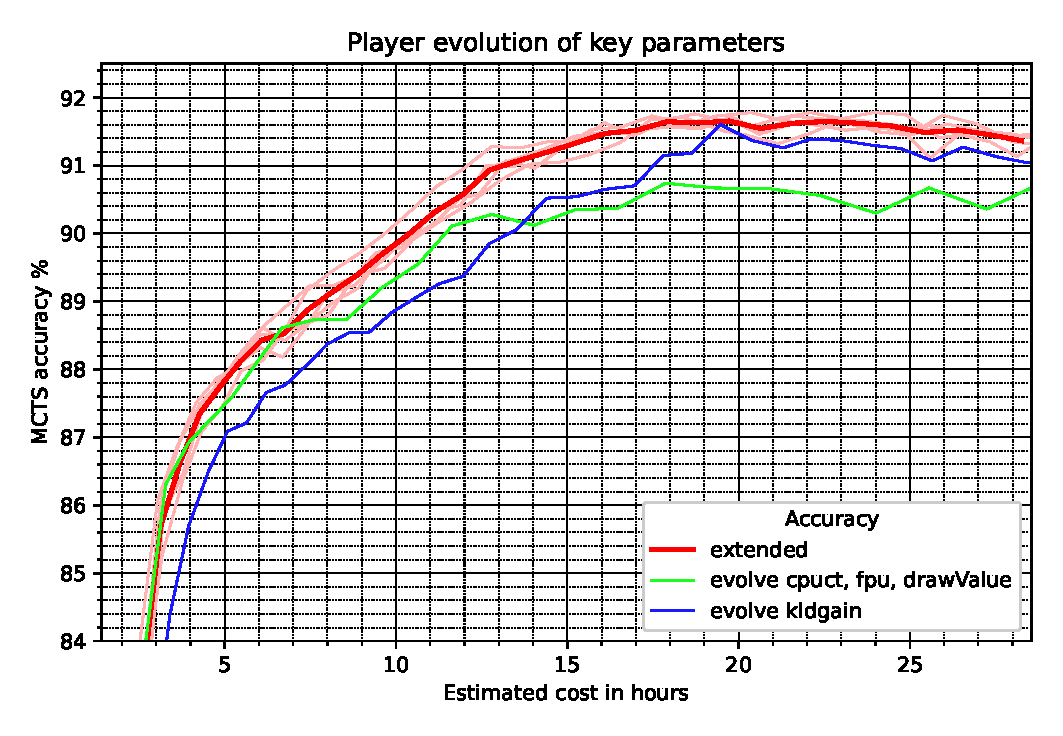
\includegraphics[clip,width=\columnwidth]{evolve_results}
\caption{Initial results of evolving hyperparameters.}
\label{fig:evolve_results}
\end{figure}

\subsubsection{Experiments}

The evolutionary approach was implemented and initial experiments run, one evolving cpuct, fpu and drawValue, the other the Kullback-Leibler divergence threshold for play with a dynamic number of MCTS nodes.
Results can be seen in figure \ref{fig:evolve_results}. Neither approach produced promising results, under-performing the baseline by a margin much larger than the run-to-run difference within the baseline.


One potential issue can be seen for the evolution of the MCTS hyperparameters in figure \ref{fig:evolve_low_diversity}, which shows a substantial drop in game play diversity when evolving those parameters.

\begin{figure}[H]
\centering
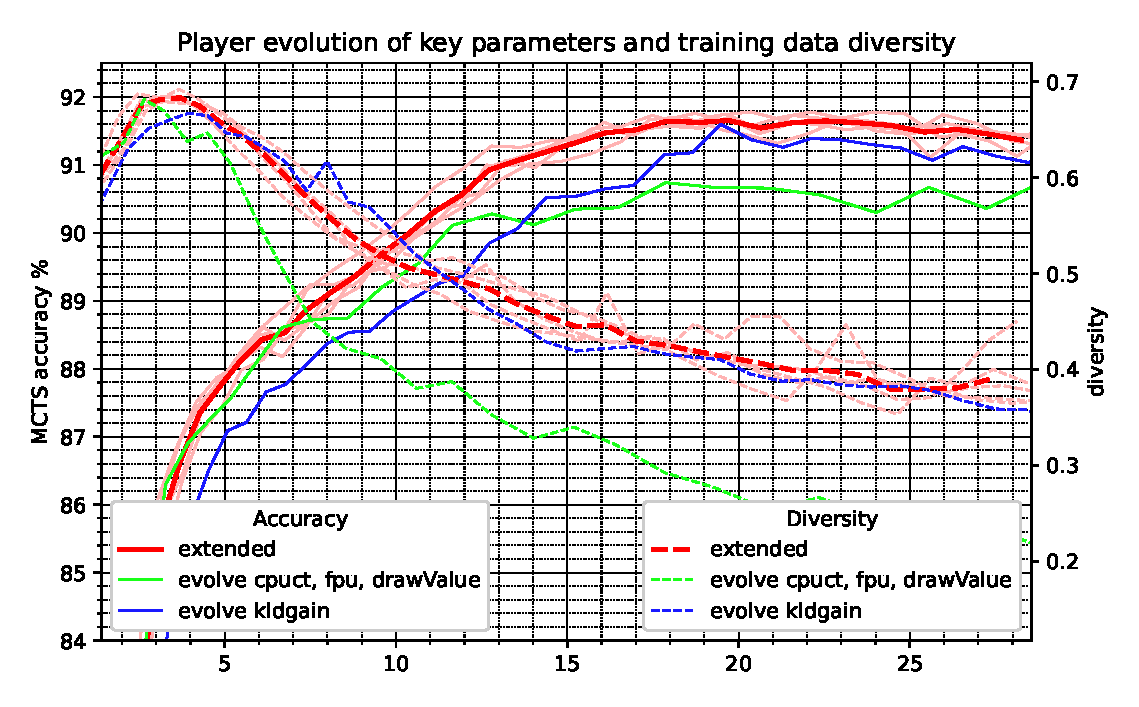
\includegraphics[clip,width=\columnwidth]{evolve_low_diversity}
\caption{Evolving basic MCTS parameters results in much lower game diversity, evolving the KL divergence threshold stays similar to the baseline. }
\label{fig:evolve_low_diversity}
\end{figure}

\subsubsection{Requirements for evolution to succeed}

First experiments with evolving players do not show good results, raising the question of what conditions have to be fulfilled to improve training efficiency with the evolutionary process.
Two key points can be established:

\begin{itemize}
 \item The player league needs to be able to pick players that actually maximize playing strength.
 \item Players that win a lot of games against other players should correspond to players that produce a high accuracy of play compared to the Connect 4 solver.
\end{itemize}

To investigate if the player evolution is able to find ''strong`` players tests were done with another hyperparameter, which was designed only for this purpose, the inversion-hyperparameter $\mathbf{I}$.
$\mathbf{I}$ modifies the move distribution found by MCTS in a way designed to disrupt playing strength.

If $m$ is the vector that represents the move distribution produced by MCTS, then the new move distribution is calculated by the inversion parameter as shown in formula \ref{eq:inverted_mtcs}.
In words: the inversion parameter controls a linear interpolation between the original move distribution and a vector that is one minus the original move distribution. Therefore, when $\mathbf{I}$ is $1$, the MCTS will produce results which put most weight on moves that originally
were considered to be the worst moves, while the best moves will receive the lowest weight. $\mathbf{I}$ should be $0$ to not disturb the MCTS results at all, giving a known optimal value towards which evolution should optimize.

\begin{equation}
 m_\text{inverted} = \mathbf{I}((1 - m) / \sum(1 - m)) + (1 - \mathbf{I}) m \label{eq:inverted_mtcs}
\end{equation}

As a first test of the players league evolution concept, it is tested how well this parameter is optimized towards zero. For this runs of $10$ player generations are done, evolving $\mathbf{I}$ in the range between $0$ and $1$.
Table \ref{t:inversion_results} shows the development of the average players over generation $3$ to $10$, as a mean of $3$ runs. Earlier generations were not recorded, because only generations after network iteration $1$ are stored.
To gain further insight into how strong the optimization is in face of reduced impact of the parameter, two more sets of $3$ runs were made, were the inversion was only applied at random with a probability $p$. $p$ was chosen to be $0.25$ and $0.05$, so in the most extreme case,
only $1$ in $20$ moves would be affected.

The results show that the evolution of players works and can pick parameters that play stronger, even in face of a lower influence of the hyperparameter on game results, such as with $p = 0.25$ or even $p = 0.05$.
Full training runs typically go for $30$ to $50$ generations, so they have even more generation to optimize parameters.

\begin{table} [H]
 \centering
  \begin{tabular}{ l | c c c }
  Generation & $\mathbf{I}$, $p = 1$ & $\mathbf{I}$, $p = 0.25$ & $\mathbf{I}$, $p = 0.05$ \\
  \hline
  3 & $0.149$ & $0.269$ & $0.446$ \\
  4 & $0.084$ & $0.217$ & $0.380$ \\
  5 & $0.071$ & $0.172$ & $0.383$ \\
  6 & $0.052$ & $0.150$ & $0.307$ \\
  7 & $0.047$ & $0.109$ & $0.290$ \\
  8 & $0.038$ & $0.106$ & $0.244$ \\
  9 & $0.029$ & $0.091$ & $0.243$ \\
  10 & $0.027$ & $0.085$ & $0.248$ \\
  \end{tabular}
  \caption{Results of optimizing the inversion hyperparameter. The evolution works, $\mathbf{I}$ is reduced substantially over the generations.}
  \label{t:inversion_results}
\end{table}


After establishing that the evolution does work in general to optimize parameters, now it is important to also establish how well such players do in the context of accuracy compared to the Connect 4 solver.

For this purpose three sets of MCTS hyperparameters are compared: The hyperparameters used in the extended AlphaZero baseline, the hyperparameters found by evolution and a set of MCTS hyperparameters, which were found by running $65$ steps of Bayesian optimization
directly towards maximum accuracy compared to the solver. This is different from the Bayesian optimization used to find the hyperparameters for the AlphaZero baseline, as no full AlphaZero run is done, instead the fitness function runs MCTS directly on a set of test positions and returns
the accuracy.

The three hyperparameter sets are compared on a random network, a network after a single training iteration and the best network of the training run. Results can be seen in table \ref{t:hyperparam_accuracy}. The random network has no evolved
parameter set, as evolved parameter sets are only generated while also training a network.

\begin{table} [H]
 \centering

  \begin{tabular}{ l  c c c c }
  \multicolumn{5}{c}{\textbf{Random network}} \\
  Parameter Set & Accuracy & cpuct & drawValue & fpu \\
  \hline
  Evolved Player & - & - & - & - \\
  Baseline & $0.6227$ & $1.545$ & $0.6913$ & $0.8545$ \\
  Bayesian Opt. & $0.6712$ & $0.08295$ & $0.106$ & $0.9995$ \\
  \end{tabular}
 
 \begin{tabular}{ l c c c c }
 \\
  \multicolumn{5}{c}{\textbf{Network iteration 1}} \\
  Parameter Set & Accuracy & cpuct & drawValue & fpu \\
  \hline
  Evolved Player & $0.7415$ & $0.5328$ & $0.8753$ & $0.9912$ \\
  Baseline & $0.7512$ & $1.545$ & $0.6913$ & $0.8545$ \\
  Bayesian Opt. & $0.7613$ & $0.8162$ & $1.0$ & $0.5255$ \\
  \end{tabular}
  
 \begin{tabular}{ l c c c c }
 \\
  \multicolumn{5}{c}{\textbf{Best network iteration}} \\
  Parameter Set & Accuracy & cpuct & drawValue & fpu \\
  \hline
  Evolved Player & $0.9068$ & $0.2925$ & $0.4728$ & $0.1411$ \\
  Baseline & $0.906$ & $1.545$ & $0.6913$ & $0.8545$ \\
  Bayesian Opt. & $0.9117$ & $0.9045$ & $0.4498$ & $0.000977$ \\
  \end{tabular}
  
  \caption{Various hyperparameters show different accuracy. Directly optimizing for accuracy shows that neither the baseline, nor the evolutionary hyperparameter perfectly capture correct play.}
  \label{t:hyperparam_accuracy}
\end{table}

These results provide multiple interesting insights:

\begin{itemize}
 \item Once the training run has reached the best network the evolved player has found a parameter set which performs equally good to the baseline parameters, however it starts weaker.
 \item Neither the baseline nor the evolved player reach the performance of a hyperparameter set only optimized to reach highest accuracy.
 \item The optimized parameter set shows how different hyperparameters are good for different phases of the training. Especially the fpu changes drastically, from the maximum possible value of $1$ to the minimum possible value of $0$. It seems
 setting cpuct low, but fpu high is an efficient way to explore with a random network. Similarly, the drawValue also starts at a higher value and is reduced later in the training run. The evolved player does capture both of these developments over the run,
 reducing the drawValue and the fpu once the best network is generated. Evolution however prefers lower cpuct values.
\end{itemize}


Lastly the three hyperparameter sets are compared in matches of $1000$ games against each other, to determine which sets actually win the most games when playing against each other using the same network. Games are played by picking a move according
to the probability distribution produced by MCTS at random.
For the evolution approach to actually improve learning efficiency, a player that wins most games should be the same as a player with a high MCTS accuracy, or else the win rate of the hyperparameters is not a good proxy for faster training progress.
Table \ref{t:hyperparam_games} shows the results of the matches between the different hyperparameter sets.

\begin{table} [H]
 \centering

  \begin{tabular}{ c c }
  \multicolumn{2}{c}{\textbf{Random network}} \\
	      VS & Baseline  \\
  \hline
  Bayesian Opt. & $625W, 360L, 15D$
  \end{tabular}
 
  \begin{tabular}{ c c c c }
  \\
  \multicolumn{4}{c}{\textbf{Network iteration 1}} \\
	      VS & Bayesian Opt. & Baseline & Evolved Player  \\
  \hline
  Bayesian Opt. & - & $581W, 366L, 53D$ & $380W, 526L, 94D$ \\
  Baseline &  $366W, 581L, 53D$ & - & $291W, 665L, 44D$ \\
  Evolved Player & $526W, 380L, 94D$ & $665W, 291W, 44D$ & - \\
  \end{tabular}
  
  \begin{tabular}{ c c c c }
  \\
  \multicolumn{4}{c}{\textbf{Best network iteration}} \\
	      VS & Bayesian Opt. & Baseline & Evolved Player  \\
  \hline
  Bayesian Opt. & - & $590W, 238L, 172D$  & $388W, 422L, 190D$ \\
  Baseline & $238W, 590L, 172D$ & - & $155W, 557L, 288D$  \\
  Evolved Player & $442W, 388L, 190D$ & $557W, 155L, 288D$ & - \\
  \end{tabular}
  
  \caption{Results of $1000$ games between different players. Results are from the perspective of the player in the row against the player of the column. The evolved player wins every single match.}
  \label{t:hyperparam_games}
\end{table}

The high win rate of the evolved player shows that the hyperparameter optimization has achieved what its optimization goal requires: Win more games. It appears this is not necessarily the same as playing in such a way as to play correct according to the Connect 4 solver
and is also not generally helpful to speed up the training processes.

Most likely this is the core reason why the evolution approach does not help efficiency: The win-rate of hyperparameters in playing against each other using the same network is not a good proxy for learning progress of AlphaZero.


\subsubsection{Novelty search as an optimization target}

Since the win-rate of players does not appear to be a good optimization target, it might be useful to instead optimize towards a novelty search objective. Novelty search has been shown before to be a useful optimization target to solve RL problems in Deep Learning as well
as evolutionary approaches \cite{lehman2011abandoning, jackson2019novelty}.

Figure \ref{fig:evolve_low_diversity} established that optimizing for winning games causes MCTS hyperparameters to be selected which reduce the game diversity substantially, which is likely to hurt exploration.
As a compromise it is proposed to replace the Elo league with a points-based league where the winner of a game is given points for every new position in a won game. Therefore a hyperparameter set has to not just win games, but win them in novel ways.
This might help to increase the game diversity. Apart from the different objective, the player-league implementation stays unchanged. Figure \ref{fig:player_evolution_win_novelty} shows that optimizing novel ways in this way does
not substantially increase game diversity, only in the later part of the training a minimally higher game diversity seems to be created. Since players still have to win to gain points they still mainly focus on winning games, as a $1000$ game match between the novelty-evolved player
and the extended baseline parameters shows, see Table \ref{t:novel_win_fail}.

\begin{figure}[H]
\centering
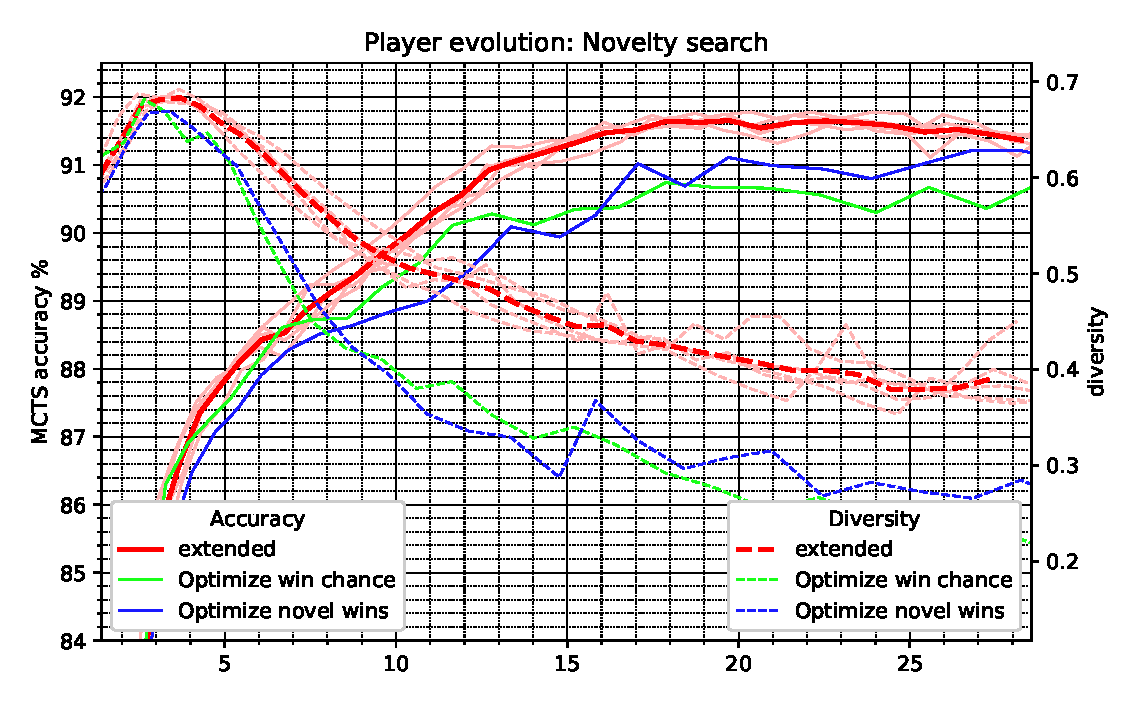
\includegraphics[clip,width=\columnwidth]{player_evolution_win_novelty}
\caption{Novelty search for novel ways to win the game shows little difference to just optimizing for wins.}
\label{fig:player_evolution_win_novelty}
\end{figure}

\begin{table} [H]
 \centering

  \begin{tabular}{ c c }
  \multicolumn{2}{c}{\textbf{Match using fully trained network}} \\
	      VS & Baseline  \\
  \hline
  Evolved & $599W, 238L, 163D$
  \end{tabular}
  
  \caption{Rewarding novel wins instead of just wins makes no substantial difference, players foremost still get optimized towards winning games. Results are from the perspective of the player in the row against the player of the column.}
  \label{t:novel_win_fail}
\end{table}

Finally, it is possible to abandon the idea of rewarding winning at all and optimize for novelty alone. This means both players get points at the end of the game, one for every novel position encountered in the game. $3$ runs were done using this optimization target,
results are shown in Figure \ref{fig:pure_novelty_search}. Towards the second half of the training game diversity is very clearly better than with the baseline, however game play performance lags substantially behind.
In the first half of the training the baseline produces more game diversity, likely because the evolution needs some time to find good parameters, while the baseline starts with parameters that were already optimized to produce good results.
The only small advantage in game diversity, even in the later half of training, indicates that the baseline parameter optimization already considered game diversity, there is not much space for improvement.

\begin{figure}[H]
\centering
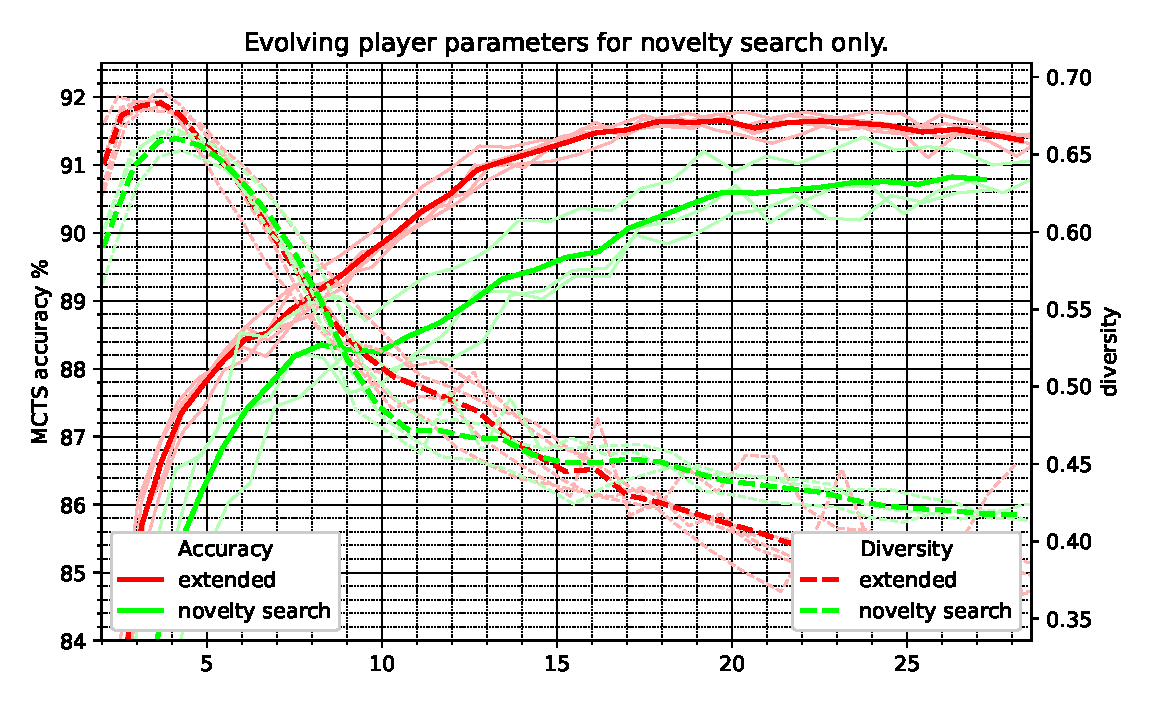
\includegraphics[clip,width=\columnwidth]{pure_novelty_search}
\caption{Even pure novelty search only produces more novel games towards the end of the training, the baseline parameters likely were already implicitly optimized for game diversity by the initial Bayesian hyperparameter optimization aiming to learn efficiently.}
\label{fig:pure_novelty_search}
\end{figure}


This closes the investigation on the evolutionary optimization of hyperparameters. No meaningful improvements could be found. However the evolution of hyperparameters by using self-play has been shown to work,
so future work might be able to identify better optimization targets that align better with the overarching goal of AlphaZero training.


\subsection{Playing games as trees}

The standard AlphaZero implementation explores new possible moves mainly by the randomization of moves, according to the policy found by MCTS.
This thesis investigates an alternative scheme of exploration, by instead playing out games in a structure similar to a tree.

A first option to do this involves to reset games to a position in which the losing player likely made a mistake and try out a different move from that position.

Another option is to abandon the idea of playing independent games to explore entirely and instead focus on playing one large MCTS-tree, which explores the current space of gameplay possibilities by the MCTS algorithm.

\subsubsection{Implementation}

To better control the games played, all games are played out on a single machine. To still scale to many GPUs, a MCTS evaluation service is created. The one machine playing the games queues positions to be evaluated and waits for
the results to return. To fully utilize a lot of GPUs, many thousands of games are played concurrently. The machine playing the games caches the MCTS search results for positions and only queues every position once per network iteration. This 
way of implementing AlphaZero increases the efficiency of GPU usage, as it prevents duplicate MCTS on common game positions. It is however only an implementation detail and cannot be considered an improvement to the algorithm.
This also changes the way the training costs are measured, to simplify the measurement of the time to play a single move, the costs are measured in the MCTS evaluation service, so the cost is calculated as the number of requested evaluation multiplied
by the cost to do a single evaluation on the ''standard`` machine.


\begin{figure}[H]
\centering
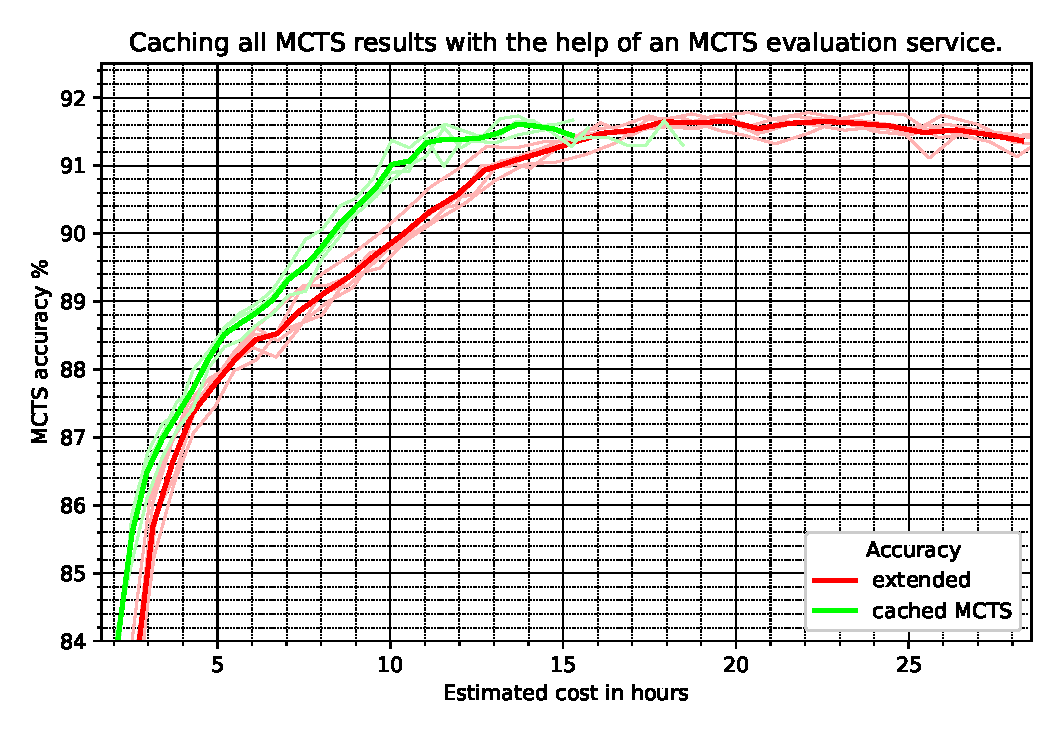
\includegraphics[clip,width=\columnwidth]{cache_play}
\caption{The MCTS evaluation service is a more efficient implementation of AlphaZero.}
\label{fig:cache_play}
\end{figure}


Since this different implementation is more efficient compared to the standard baseline normal training runs are done using the MCTS evaluation service with no further changes in the algorithm to establish a new baseline.
Any algorithmic improvements which need the MCTS evaluation service are compared against this new baseline. The baseline is compared with the previously defined extended baseline in Figure \ref{fig:cache_play}.



\subsubsection{Resetting games to a position before a likely mistake}

This idea aims to explore by trying out to play another move in a position that might have been the reason a game was lost.

Randomized play is reduced to the first $16$ turns of a game, down from $30$, to focus exploration on the novel way investigated here.
Instead of relying on randomized moves to explore, once a game is completed it is reset to an earlier position and replayed with a different choice of moves from there. This choice of moves is intended to be done in a way that explores new gameplay possibilities.

The suggested way to choose a new move is to first search the position in which the predicted chance to win of the losing player dropped the most compared to before the latest move was made. For this the position value prediction of the network is used.
This should indicate a position in which a likely bad move was played.


\begin{figure}[H]
\centering
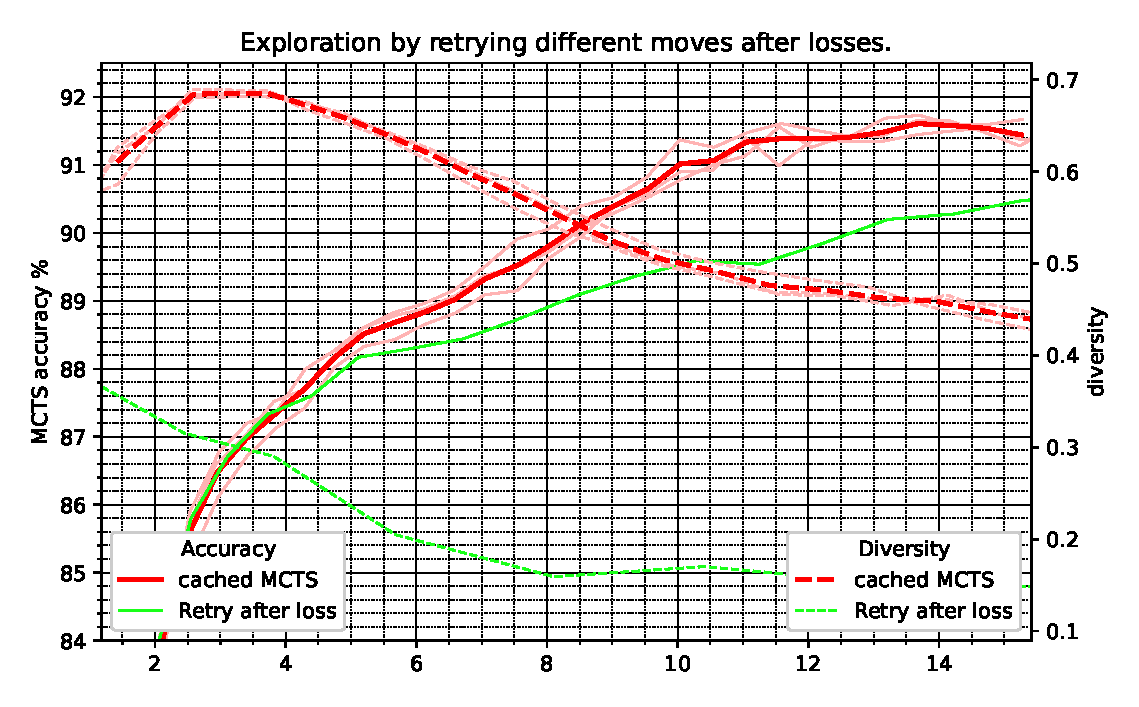
\includegraphics[clip,width=\columnwidth]{winp_tree}
\caption{Retrying a different move  in a critical position to explore does not appear to work.}
\label{fig:winp_tree}
\end{figure}

From one position earlier, before the network value evaluation dropped, a new game is started and lets the loosing player pick the best move in the position that has not been played yet.
This way the player who lost a game gets another attempt to rectify a mistake that might have lead to the loss, exploring a new branch of the game tree that potentially represents better play.


Figure \ref{fig:winp_tree} shows results of this idea. The results are not good, it appears the randomized moves are substantially better at exploration, with game diversity drastically reduced when exploring by retrying a different move in a critical position.



TODO maybe do another run with the exploration set back to up to turn 30 and another with turn 0?

\subsubsection{Explore the game tree in the same fashion as MCTS}

The exploration-exploitation dilemma faced by AlphaZero self-play is the same one that MCTS aims to solve. It might thus make sense to explore the game tree by MCTS instead of randomized self-play.
Specifically it is proposed to create a tree of game position, by MCTS rules, to generate example games and game results. Since AlphaZero needs to scale to many distributed machines, virtual losses \cite{chaslot2008parallel} are used to play out many games 
using the same MCTS tree. This should not be confused with the MCTS used to evaluate single game positions. That per-position MCTS is still used to evaluate positions, effectively stacking two MCTS searches into each other. The one big MCTS that generates training data
and replaces randomized self-play uses the per-position MCTS as position evaluations, just like the per-position MCTS uses the neural network.

A virtual loss is given to every node visited, pushing following games to investigate other nodes if too many such losses push down the value of a node in the search tree.
Every game played represents one thread walking down the tree, adding virtual losses to visited nodes. Unlike in AlphaZero MCTS, games have to be played out to a final result before backpropagation can occur. 

To fully utilize ten or more GPUs, thousands of games have to be played in parallel. This might prove a challenge to 
the virtual loss concept, as the original paper proposing virtual losses tested with only up to $16$ threads, whereas in this case thousands will be necessary.

Another challenge is the exchange of the network once a new network has been trained. This makes it necessary to reevaluate all positions in the tree. If one is not careful, this can substantially increase the training cost,
as lots of positions have to be evaluated every time a new network is trained before any new game results can be reported, since games have to all start from the first turn again. A game can only be reported once it has been played through fully,
so if a game is half completed when a new network is created there is the choice between throwing away the game, since it is based on an old network, or accepting the game reports into the training data anyway. 

Throwing away the MCTS tree when a new network 
is completed would implement throwing away the half finished games, which is too expensive.
Even after a new network has been trained, games that finish with positions only evaluated by the previous network are still reported. Instead of throwing away the MCTS tree, nodes are only reevaluated as they are encountered again,
with currently running games untouched.
This is similar to how normal AlphaZero might report some game states to the training server that use an older network due to the distributed nature of the workers.

One more difference with the MCTS implementation to discover new gameplay is that it uses a hash table between game position and tree nodes. This way, for every game position only a single node can exist, handling game transpositions in a rudimentary way. For 
the backpropagation of game results transpositions are ignored however and only the recently played path from the root is back-propagated over.

Experiments with this self-play approach quickly revealed that MCTS tends to get stuck on a relatively low number of possible games, dropping game diversity and hurting exploration. 
Figure \ref{fig:mcts_tree_explore} shows that even setting the exploration-exploitation hyperparameter cpuct of the MCTS to extremely large values up to $15$ does not help against this.
Increasing game diversity stays out of reach entirely.

\begin{figure}[H]
\centering
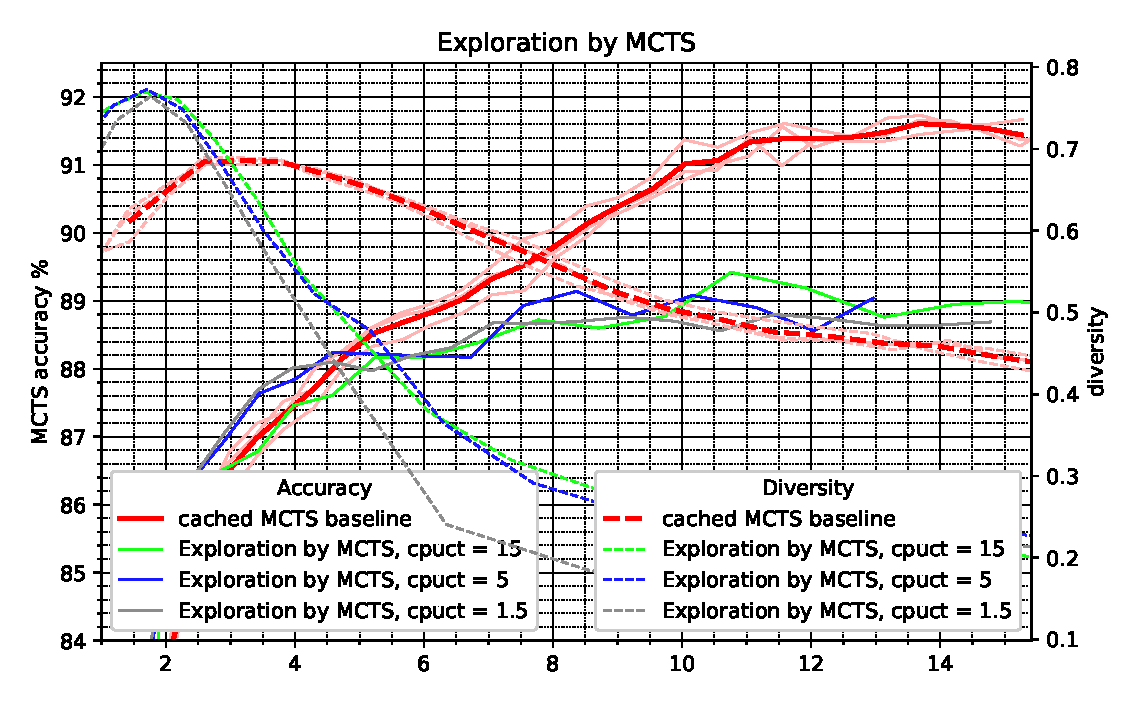
\includegraphics[clip,width=\columnwidth]{mcts_tree_explore}
\caption{Replacing self-play with one large MCTS. MCTS tends to get stuck on a few paths of games and stops exploring, reducing the diversity of game positions encountered.}
\label{fig:mcts_tree_explore}
\end{figure}


\subsection{Using network internal features as auxiliary targets}

\cite{wu2019accelerating}[Wu et. al.] shows that using domain specific features as auxiliary targets to regularize learning improves learning in Go. This motivates the search for an automatic way to find such targets.

This thesis proposes to use internal feature representations of a small network, shown in Figure \ref{fig:sq_bottleneck_network}, to be used as such auxiliary targets. For this purpose a full AlphaZero run is done, learning to play Connect 4 using a very small network with less than $70000$ 
parameters, a fraction of the $1.5$ million parameters of the network used in all other experiments. This small network uses only a single filter in the last convolutional layer for both output-heads of the network. The prediction of the policy as well as the prediction of the game outcome 
are bottlenecked by only $42$ features each, one feature for each of the $6 \times 7$ fields of Connect 4.

Training such a small network to an accuracy of about $84\%$ takes about two hours of computational time on a single GPU. The network can afterwards be used to generate features when training in an AlphaZero run with a larger network.
Multiple options exist on how to use these features exactly. First a distinction can be made between the features of the game outcome prediction, the win-features, and the features of the policy prediction, the move-features.

For a given training example, the small network is run on it to produce these feature sets, producing the features of the present position. Additionally more features can be generated by considering future positions that occurred in the game
after a training position. This defines the future-features, which may induce the ability to predict the future of a game position in the regularized network. In this thesis future positions $2$ and $4$  ply in the future are considered.
Including the present position this gives up to three feature layers to be used as regularization targets. They are named move0 to move2 and win0 to win2, $0$ standing for the present, $2$ for the $4$ ply future features. move1 and win1 also include respectively move0 and win0,
move2 and win2 include all layers. Additionally it was tried to only regularize with some of the future feature layers and not the earlier ones, this is named only move1 to only move2 and only win1 to only win2.

To regularize the bigger network a mean square error is used to add to the training loss, calculating the mean square error between the auxiliary feature and an internal layer of the big network. No additional parameters are added to the bigger network,
only some internal layers are enforced to produce the auxiliary features. Two options are investigated: Regularize the very last convolutional layer and regularize the output of the last residual network block. The last convolutional layers before
the fully connected output layers have $32$ filters in the big network, so even when learning $4$ to produce the regularization target it leaves $28$ for arbitrary representations. The last residual network block has $128$ filters, so again only a small number is regularized.


\begin{table} [H]
 \centering
  \begin{tabular}{c | c }
   Description & Network structure \\
   \hline
   \hline
   Initial block & $\begin{pmatrix} 3 \times 3 \times 128 \\ BatchNorm \\ ReLU \end{pmatrix}$ \\
   \hline
   Adapter convolution & $1 \times 1 \times 32$ \\
   \hline
   SQ residual block, repeated $3$ times & $\begin{pmatrix} 3 \times 3 \times 32 \\ BatchNorm \\ ReLU \\ 3 \times 3 \times 32 \\ BatchNorm \\ AVG Pooling \\ FCnb: 4 \\ ReLU \\ FCnb: 32 \\ Sigmoid \\ Addition \\ ReLU \end{pmatrix}$ \\
   \hline 
   Move policy output & $\begin{pmatrix} 3 \times 3 \times 1 \\ FC: 7 \\ SoftMax \end{pmatrix}$ \\
   \hline
   Win prediction output & $\begin{pmatrix} 3 \times 3 \times 1 \\ FC: 3 \\ SoftMax \end{pmatrix}$
  \end{tabular}
  \caption{The small bottleneck network used as a source of auxilary learning targets. The network has about $70000$ parameters.
  The network primarily has much less parameters, as it uses only $32$ filters throughout the residual blocks, instead of $128$. The outputs both are based on a convolution with a single filter, yielding $42$ features for each the win prediction and the move policy. Those $42$
  features are used as auxilary features for game positions and learnt by the bigger network as a regularizer.}
  \label{fig:sq_bottleneck_network}
\end{table}



To first establish where various combinations of these options might stand, supervised training is enhanced with the auxiliary features. Results are shown in Table \ref {fig:supervised_results_auxilary_f}. It can be seen that regularizing with the features of the
move output produces very small improvements outside of the standard deviation of the runs. Using the win features worsens the results of supervised training.

\begin{table} [H]
 
  \centering
  \begin{tabular}{c | c | c}
   configuration & accuracy moves & accuracy wins \\
   \hline
   \hline
   Baseline, no auxilary features & $92.6\% \pm 0.1$ & $78.94\% \pm 0.1$ \\
   \hline
   move0 & $92.76\% \pm 0.1$ & $78.98\% \pm 0.06$ \\
   \hline 
   win0  & $91.45\% \pm 2.23$ &  \boldmath{$79.98\% \pm 2.04$} \\
   \hline
   move0, win0 & $92.81\% \pm 0.08$ & $78.96\% \pm 0.06$ \\
   \hline
   move1 &  \boldmath{$92.89\% \pm 0.07$} & $79.09\% \pm 0.06$ \\
   \hline
   win1 & $92.51\% \pm 0.05$ & $78.82\% \pm 0.07$ \\
   \hline
   move2 & $92.80\% \pm 0.05$ & $78.99\% \pm 0.06$ \\
   \hline
   win2 & $92.35\% \pm 0.02$ & $78.75\% \pm 0.06$ \\
   \hline
   only move1, only win 1 & $92.57\% \pm 0.06$ & $78.86\% \pm 0.05$ \\
   \hline
   only move2 & $92.79\% \pm 0.05$ & $79.05\% \pm 0.11$ \\
   \hline
   only win2 & $92.41\% \pm 0.12$ & $78.81\% \pm 0.11$ \\
   
   
  \end{tabular}
  \caption{Supervised results for auxilary features. Mean and standard deviation of $5$ supervised runs, using the same setup as in section \ref{sec:supervised} on page \pageref{sec:supervised}}
  
  \label{fig:supervised_results_auxilary_f}
  
\end{table}

Since the differences are only quite small another set of supervised experiments was done using the easier dataset with only $10\%$ random moves played during dataset generation, as described in section \ref{s:generate_dataset} on page \pageref{s:generate_dataset}.
Results mirror the results of the harder dataset, again move1 shows the most improvement, again only a very small difference, albeit outside of the standard deviation of the runs.

\begin{table} [H]
 
  \centering
  \begin{tabular}{c | c | c}
   configuration & accuracy moves & accuracy wins \\
   \hline
   \hline
   Baseline, no auxilary features & $96.94\% \pm 0.02$ & $84.75\% \pm 0.04$ \\
   \hline
   move0  & $97.04\% \pm 0.05$ & $84.79\% \pm 0.03$ \\
   \hline 
   win0  & $96.08\% \pm 1.5$ & $83.89\% \pm 1.15$ \\
   \hline
   move0, win0 & $97.04\% \pm 0.071$ & $84.71\% \pm 0.05$ \\
   \hline
   move1 &  \boldmath{$97.16\% \pm 0.04$} &  \boldmath{$84.81\% \pm 0.03$} \\
   \hline
   win1 & $96.89\% \pm 0.04$ & $84.66\% \pm 0.05$ \\
   \hline
   move2 & $97.10\% \pm 0.05$ & $84.73\% \pm 0.02$ \\
   \hline
   win2 & $96.79\% \pm 0.09$ & $84.58\% \pm 0.04$ \\
   \hline
   only move1, only win 1 & $97.00\% \pm 0.08$ & $84.71\% \pm 0.04$ \\
   \hline
   only move2 & $97.04\% \pm 0.07$ & $84.75\% \pm 0.03$ \\
   \hline
   only win2 & $96.91\% \pm 0.07$ & $84.67\% \pm 0.05$ \\
   
   
  \end{tabular}
  \caption{Supervised results for auxilary features on easy dataset. Mean and standard deviation of $5$ supervised runs, using the same setup as in section \ref{sec:supervised} on page \pageref{sec:supervised}, 
  with the easier dataset as described in section \ref{s:generate_dataset} on page \pageref{s:generate_dataset}}
  
  \label{fig:supervised_results_auxilary_f_easy_dataset}
  
\end{table}

Following from these results move1 has been picked as the best candidate for a successful AlphaZero run. Additionally however experiments have also been run with a few other configurations, to verify if supervised results to correspond with AlphaZero results. 
win0 was chosen because of its unstable results in supervised, combined move0 and win0 because of how close they were to move1 and finally only move2 was chosen to include a configuration as far as possible in the future.
In the following data the cost of the runs with auxiliary features has been increased by a $2$ hours to include the training of the network used as a source of features. Results are shown in Figure \ref{fig:auxiliary_attempt1}.

\begin{figure}[H]
\centering
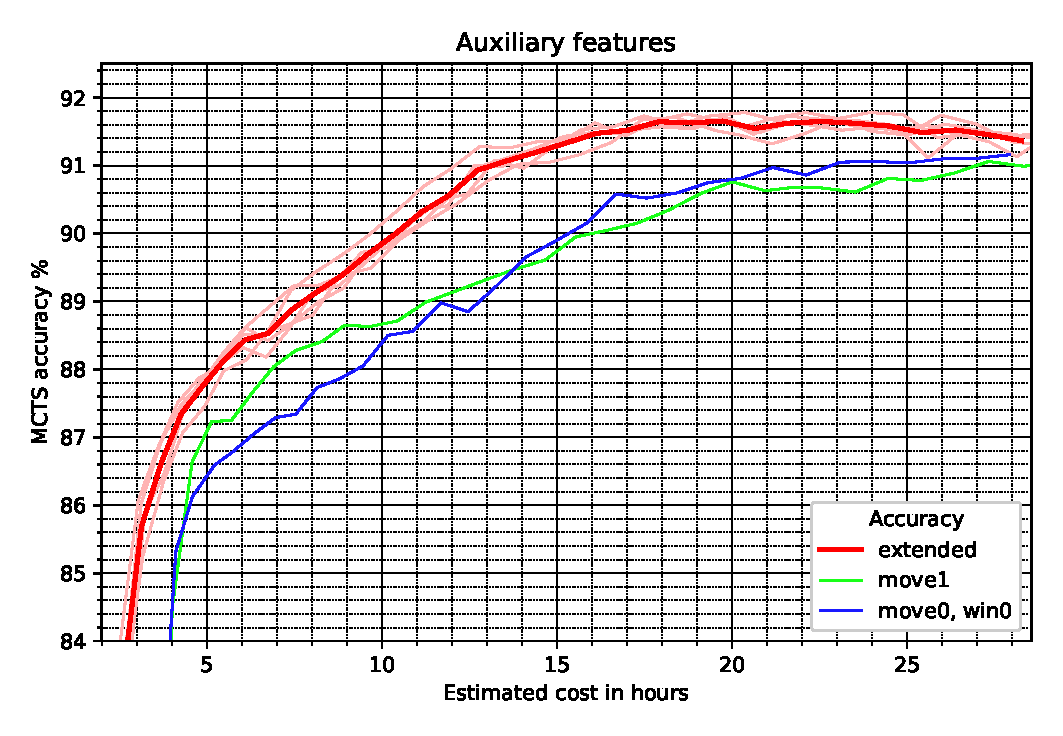
\includegraphics[clip,width=\columnwidth]{auxiliary_attempt1}
\caption{Using auxiliary features from a smaller network with AlphaZero.}
\label{fig:auxiliary_attempt1}
\end{figure}

Results are not very promising. Whereas in the supervised setting the final accuracy was slighly higher, here it is actually lower. The extra cost of $2$ hours of time to train the initial network pushes the cost up a lot and makes the use of auxiliary features like this not worthwhile.
The first few iterations however do show a faster rise in accuracy when the extra costs are ignored, as shown in Figure \ref{fig:rndVsTrainedAux}. Even without the issue of the extra costs, the baseline reaches a substantially higher final result.
An interesting result is found when using a random network for auxiliary features, also shown in Figure \ref{fig:rndVsTrainedAux}, instead of one trained in a previous AlphaZero run. This reduces the costs for initialization to $0$. The training run with random features follows the extended baseline very closely.
It seems to fall off minimally towards the end, but that might just be run-to-run variance. 

\begin{figure}[H]
\centering
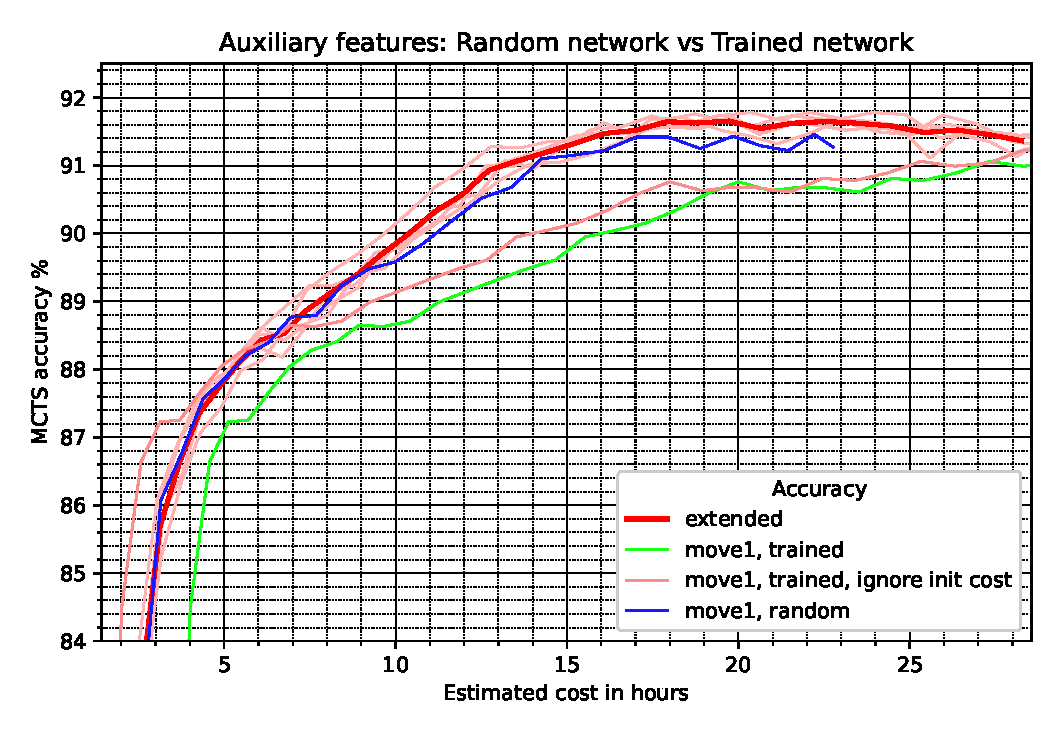
\includegraphics[clip,width=\columnwidth]{rndVsTrainedAux}
\caption{The training costs of the feature network push the auxiliary feature-enhanced training run behind the baseline.}
\label{fig:rndVsTrainedAux}
\end{figure}



In summary using a pre-trained smaller network for features does appear to help at the beginning of the training, but not enough to pay for the costs of training the network. Additionally the performance in later parts of the training is held back, likely by the
regularization that keeps enforcing the auxiliary features which are only useful for prediction on an accuracy level of about $84\%$.

This raises the questions: Can the initial cost be reduced? Can the negative influence in the later parts of the training be prevented?

An important observation related to these questions is that the training of the smaller network, which was used for the features, reached $84\%$ in just $2$ hours of training. This is a lot faster than the baseline, which requires about $3$ hours.
Starting training with a smaller network and then switching over to a bigger network does in fact raise learning efficiency, as can be seen in Figure \ref{fig:growNetwork}. Specifically the number of filters in the convolutional filters is grown in this run,
starting with $16$ filters and doubling the number of filters in iteration $4$, $8$, $16$ and $32$. This means that by iteration $32$ the network will use twice as many filters as the other networks in this thesis. The switchover results in visible
drops in accuracy, which get bigger the bigger the network was. This is likely as training just a single epoch of the window of two million examples is not enough to train the bigger network back to where the previously used smaller network was.
This becomes especially visible in the last step, where the biggest network produces a sharp drop in performance. The earlier parts of the training however look very promising in terms of efficiency gains.
This is not a novel idea, growing the size of the network as its playing strength rises has been done by the LCZero project \cite{lzNetworks} as well as in other AlphaZero related works such as by \cite{wu2019accelerating}[Wu. et al].
No specific research appears to have been done however on how to maximize the effect.

\begin{figure}[H]
\centering
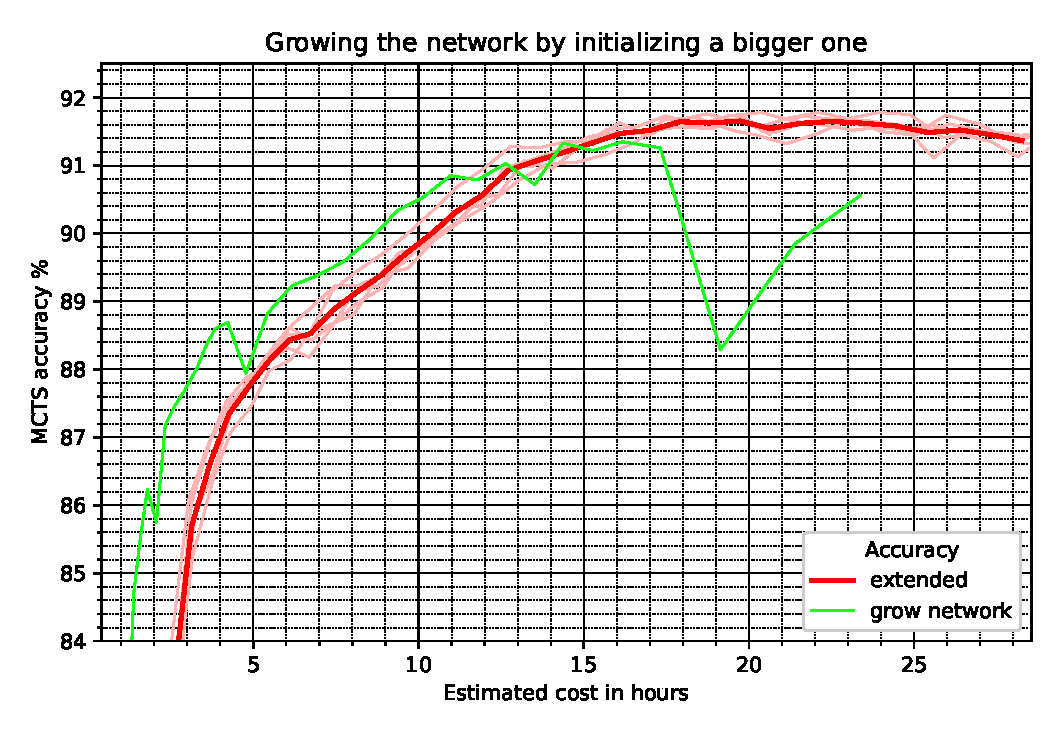
\includegraphics[clip,width=\columnwidth]{growNetwork}
\caption{Growing the network as the run progresses does increase efficiency.}
\label{fig:growNetwork}
\end{figure}

Growing the network like this has a useful side effect for the concept of auxiliary features: The smaller networks created in the earlier iterations can be used to provide auxiliary features for the later networks, at no additional training costs.
This leaves the issue of preventing the auxiliary features from holding back the bigger network, as has been shown to happen in the experiments with auxiliary features.
A possible explanation to the drop in accuracy in later parts of the training might be the layer which is regularized is directly used as in input to the output layer of the network, which might be too disruptive. To investigate, another run with auxiliary features was
made, using move1, but with an extra output head whose sole purpose are the regularization features. 





\section{Conclusion}

\begin{itemize}
 \item Establishing comparable baselines is hard, as shown on how different connect4 datasets can produce wildly different absolute values.
 \item Evolution works, but what objective to use
 \item Different modes of exploration all suck compared to plain random(). Plain random() really is incredibly good.
 \item Skipped new network stuff, gather excite, because that is just not that much better than squeeze excite and sq was already not a big jump
\end{itemize}



\pagebreak

% -- Literaturverzeichnis --------

\bibliographystyle{plain}     % nummeriere Zitate [1], [2], ...

% Quellenangaben stehen in einer separaten BibTeX-Datei Seminararbeit.bib
\bibliography{document}

\end{document}
